\documentclass[Japanese]{dicomopapers}
%\documentclass[Japanese,noauthor]{dicomopapers}
\usepackage[dvipdfmx]{graphicx}
\usepackage{latexsym}
\usepackage{url}
\renewcommand{\baselinestretch}{1.0}

\def\Underline{\setbox0\hbox\bgroup\let\\\endUnderline}
\def\endUnderline{\vphantom{y}\egroup\smash{\underline{\box0}}\\}
\def\|{\verb|}



\begin{document}

% 和文表題
%\title{BLEビーコンを用いた物体状態推定手法}
\title{物体内部に設置したBLEビーコンの\\電波強度を用いた状態推定手法}

% 英文表題
%\etitle{Proposal of Object State Estimation Method \\ using BLE Beacon}
\etitle{State Estimation Method using Radio Wave Intensity \\ of BLE Beacon installed Inside Object}

% 所属ラベルの定義
\affiliate{1}{愛知工業大学 情報科学部情報科学科}

\author{大鐘 勇輝}{YUKI OGANE}{1}
\author{水野 涼雅}{RYOGA MIZUNO}{1}
\author{梶 克彦}{KATSUHIKO KAJI}{1}




\begin{abstract}
IoTの普及によって様々なセンサが家電に取り付けられ,そこから得られる情報によりライフログデータの取得が可能となった.
ライフログデータはセンサが搭載されている家電では収集が容易であるが,特殊なセンサの無い家電や扉,椅子といった家具ではデータの収集が難しい.
これまでそのような家電や家具などの状態推定には加速度センサやWi-Fiの電波が用いられてきたが,移動の有無や推定対象物の大きさによって推定精度が大きく左右される問題があった.
そこで本研究では,Bluetooth Low Energyビーコン(以下BLEビーコンと呼称)を家電や家具などモノの中に直接入れ,状態によって変化するBLEビーコンの電波強度をもとに推定を行う手法を提案する.
BLEビーコンの電波は微弱であるため,環境の変化による電波の乱れが発生しやすい.
そのため提案手法では,取得した電波強度データに対しデジタルフィルタの一つであるローパスフィルタを適用しノイズの除去を行う.
また,本手法では推定対象物の移動も考慮するため,簡単な閾値処理だけでは推定が困難である.
そこで,安定センシング区間という概念を導入し,電波強度が安定している区間を用いて推定精度の向上を試みる.
見つかった安定センシング区間に対し動的に変更できる閾値を用いて状態推定を行う.
上記の方法を冷蔵庫の開閉や金庫の開閉,座椅子の着座の状態推定に適用し推定精度を確かめた.
その結果,冷蔵庫の開閉推定では99.2%,金庫の開閉推定では93.8%,座椅子の着座推定では98.9%の精度で推定できた.

\textgt{\\キーワード} : BLEビーコン,状態推定,安定センシング区間,ライフログ,ローパスフィルタ



\end{abstract}

% 表題などの出力
\maketitle

% 本文はここから始まる
\section{はじめに}
通信インフラの整備とIoTの発展により,現在では様々なモノがインターネットに繋がるようになった.
エアコンや照明,家の鍵から車に至るまで,数年前ではインターネットとは無関係だったものが今では当たり前のようにインターネットに接続されている.
IoTに対応した家電は遠隔からの機器の操作や機器の状態の通知,使用ログの保存が可能であり,例えばIoTに対応したエアコンでは家の外から電源のON・OFFや電気使用量のログの確認ができる.
そうした利便性から日々新たなIoT家電が生み出され続けており,総務省が公開している資料\cite{soumusyo}によると2020年には約300億のIoTデバイスが稼働していると予想されている.
IoTデバイスの増加により家中にそれらが設置されると,そこから得られる使用データから行動パターンといったライフログのデータが取得できる.
ライフログのデータは,環境に合わせた電力制御や老人の異常行動の検知など幅広い分野への応用が期待できる.

しかし,これらのデータはIoTに対応した家電でないと取得できず,金庫や椅子,扉といった家電以外のモノではセンサが無いためデータ収集が不可能という問題がある.
この解決策として,(1)加速度センサや回転センサを使う方法と,(2)Wi-Fi電波のチャネルの状態情報を使った方法がある.
(1)の方法は直接モノの動きを観測できるため安定した精度で状態推定ができる反面,センサー単体での動作が難しく取得したデータの保存・解析に専用の機器が必要である.
また,(2)の方法では対象物のそれぞれにセンサを付ける必要が無い一方,状態の推定にWi-Fi電波の反射波を用いるという特徴から小さな対象物への適用は不向きである.

そこで本研究では汎用的な機器のみで動作でき,かつ小さな対象物でも高い精度で状態推定できる手法を提案する.
具体的には日常の生活空間内における家電・家具の内部にBLEビーコンを設置し,送信される電波をスマートフォンで受信した際の受信電波強度をもとにモノの状態推定を行う.
これまでBLEビーコンは広告配信や位置推定のための電波を発する言葉通り「ビーコン」として使われてきたが,物体内部に設置し「センサ」としての使い方をされている例はあまりない.
BLEビーコンから発信される電波は微弱なため障害物の有無により電波強度が変化しやすく状態推定に適しており,省電力なため長期間の稼働が可能である.
加えて電波はスマートフォンで受信できるため,電波の受信に特別な機器を必要とせず,UUID,major,minorの情報から各BLEビーコンの識別ができるため,1台のスマートフォンで複数のBLEビーコンを監視できる.
システム概要図を図\ref{abst}に示す.
本手法では,BLEビーコンを金庫や冷蔵庫であれば開閉を行う蓋や扉の部分に,座椅子では座面のクッション下へ設置し推定を行う.
この時,受信したデータをそのまま使用するとノイズの影響により正確な推定ができないため,収集したデータに対してフィルタ処理を施し,ノイズを取り除いてから状態の推定を行う.
状態の推定には安定センシング区間という概念を利用しており,これにより推定対象物が移動したとしても状態推定が可能である.

本稿の構成は以下の通りである.
2章では,屋内日常物における状態推定に関する既存研究を紹介し,その問題点を述べる.
3章では,既存手法における問題点を解決するために,本研究のBLEビーコンを使用してモノの状態推定を行う手法を述べる.
4章では,本研究で提案した手法の評価を行う.
最後に5章・6章で,考察と本研究のまとめを行う.


%ーーーーーーーーーーーーーーーーーーーーーーーーーーーーーーーーーーーーーーーーーーーーーーーーー
%ーーーーーーーーーーーーーーーーーーーーーーーーーーーーーーーーーーーーーーーーーーーーーーーーー

% 図の挿入
\begin{figure}[tbh]
 \centering
 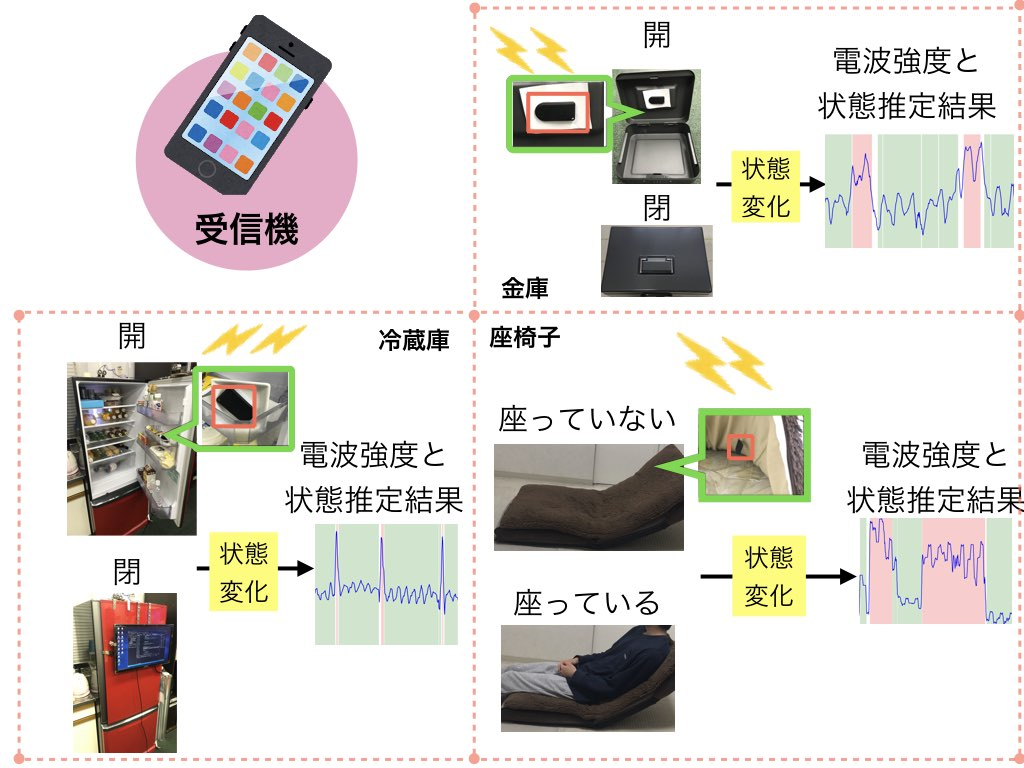
\includegraphics[width=8.5cm]{abst.jpeg}
 \caption{システム概要図}
 \label{abst}
\end{figure}

\section{関連研究}
室内にある物の状態推定には,加速度センサや振動センサなどを利用する方法やWi-Fiの電波を利用する方法など様々な手法が提案されてきた.
前川ら\cite{TagAndThink}は様々なセンサを搭載したセンサノードをモノに取り付け,そこから得られるセンサ情報と事前に用意しておいたそのモノ固有の状態遷移図を比較し,自動でモノの状態と何に付けられているのか推定をしている.
角速度や照度などから,センサノードが取り付けられている状況や状態変化を検出するという手法である.
この手法ではセンサノードがどんなモノに付いていて,どんな状態変化をしたか推定が可能である.


消費電力の変化から電気機器の状態推定を行っている研究がいくつかある.
例えば,機器やコンセントごとの消費電力を計測できる細粒度電力センサを使用し,電気機器の電力消費の変化から浪費電力の検出・分類が行われている\cite{sairyu}.
その他にも電気機器の運転モードの切り替えや開閉などの状態変化によって起こる消費電力の変化から状態の推定を行い,そこから得られる時系列の情報から人物の位置推定が行われている\cite{energy}.
これら二つの手法では,電気機器の状態変化から起こる消費電力の増減に着目し推定を行っているため,電化製品に対しては有効な手法ある.
一方で,電気を用いない家具や雑貨に対しては適用が不可能である.


日常生活空間内での扉の開閉推定を行う研究\cite{WifiChannel}では,Wi-Fiのチャンネル状態情報を用いて物体の移動から発生するドップラー効果や電波の到来方向からドアの開閉状態を検知している.
この研究では推定の対象物は扉でありある程度大きさがあるモノであるため,Wi-Fiチャネル状態情報に影響を及ぼしやすくこの手法は有効である.

しかし,小さな箱の開閉や移動した先での状態変化を推定する事は難しいため,本研究ではBLEビーコンを用いて電波強度の変化から状態変化の推定を行う.
Bluetooth Low Energyの技術は,広告配信や位置推定など様々な用途に使われている.
例えばSNSサービスを提供しているLINEでは,BLEビーコンを使用して決済ができるサービスを提供している\cite{bleUse}.
その他にもBLEビーコンの電波は,在室検知や位置推定など多くの研究に利用されている.
在室検知では各個人がBLEビーコンを持ち,室内に設置された受信機で在室を検知する研究が行われている\cite{en-AreaUsed},\cite{Finding_by_Counting},\cite{dakoku_system}.
また,BLEビーコンと受信機との距離による減衰や,障害物による電波の減衰によって変化する電波強度をもとに,複数の受信機を用いて位置の推定や状態の推定をする研究が数多く行われている\cite{IoMT},\cite{tandem},\cite{blespot},\cite{en-door}.%,\cite{LANgate},.
これらで利用されているように,BLEビーコンの電波は微弱であるため数mの距離の変化や障害物により電波強度の変化が起こる.
この現象を利用し日常の生活空間内におけるモノの状態変化の推定を行う.





%ーーーーーーーーーーーーーーーーーーーーーーーーーーーーーーーーーーーーーーーーーーーーーーーーー
%ーーーーーーーーーーーーーーーーーーーーーーーーーーーーーーーーーーーーーーーーーーーーーーーーー





\section{物体内部に配置したBLEビーコンの電波強度を用いた状態推定}
状態変化による電波強度の変化を利用した研究がいくつか行われている.
例えば,複数あるBLEビーコンの中からある一つを手で覆ったり開いたりするパカパカという動作からそのBLEビーコンを特定し,管理を容易にするという研究がある\cite{BLEpkpk}.
また無線LANの電波環境がドアやエレベータなどゲートの通過前後で大きく変わる点に着目し,ゲート通過検出を行っている研究がある\cite{BLEpkpk}.
本研究ではこれらで利用されている電波強度の大きな変化に着目する手法を取り入れる.
冷蔵庫の開閉などモノの状態変化時にはBLEビーコンの遮蔽状態が変化するため,これらで利用されているような動作前後で受信電波強度が大きく変化する現象が起こる.
そのため電波を減衰させやすい材質であればモノの状態推定が可能であると考えられる.

本研究では冷蔵庫や金庫,座椅子などの内部に図\ref{beacon}のBLEビーコンを設置し,その状態変化による電波強度の変化からモノの状態推定を行う.
冷蔵庫(図\ref{freezer})では扉の棚部分,金庫(図\ref{safe})では開閉する蓋の部分,座椅子(図\ref{chair})では人が座る座面の部分や背もたれの部分のカバー裏へBLEビーコンを設置する.
冷蔵庫や金庫では金属による電波の減衰が起き,座椅子では人体によって電波の減衰が起こる.
これにより扉の開閉や人の着座などのモノの状態変化からBLEビーコンの遮蔽状態が変化するため,外側に設置した受信機からみるBLEビーコンの電波強度が変化する.
この変化する電波強度をもとにモノの状態変化の推定を行う.





% 図の挿入
\begin{figure}[tbh]
    \centering
    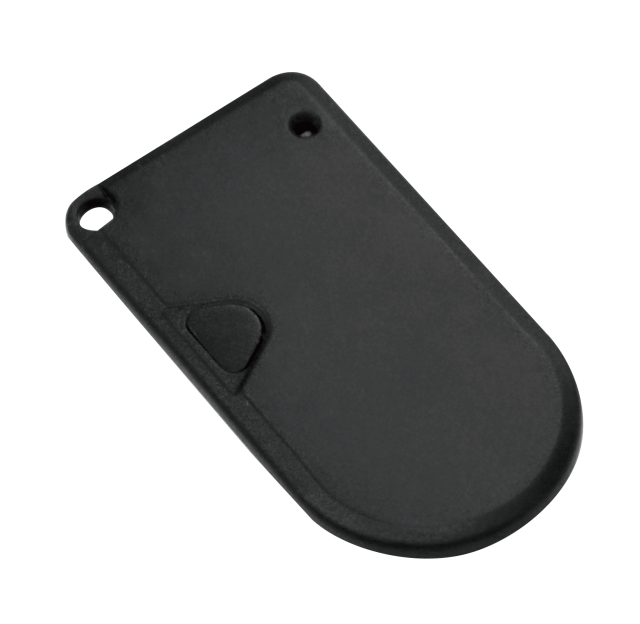
\includegraphics[width=3cm]{ble.png}
    \caption{BLEビーコン}
    \label{beacon}
   \end{figure}

\begin{figure}[tbh]
    \centering
    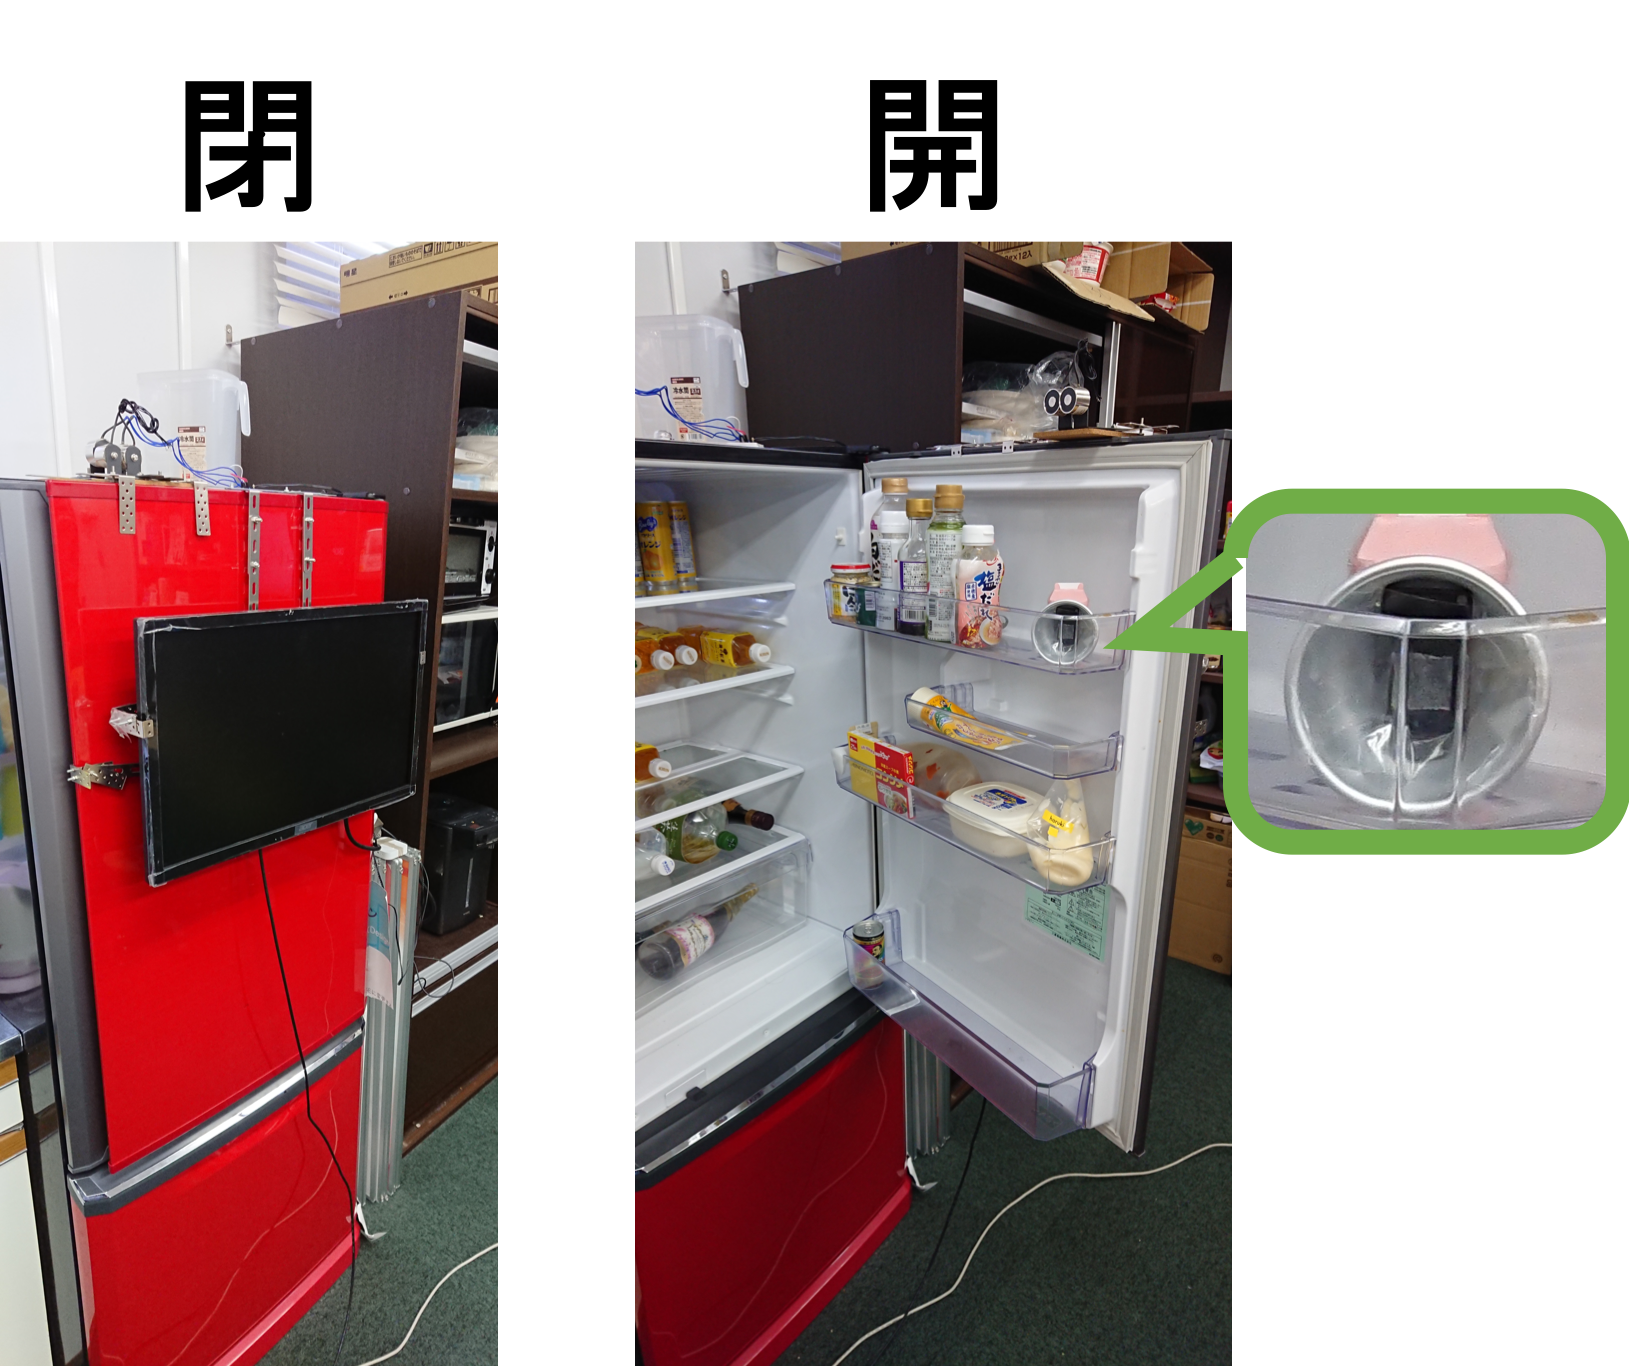
\includegraphics[width=7cm]{regisW2.png}
    \caption{冷蔵庫の状態と設置したビーコン}
    \label{freezer}
\end{figure}

\begin{figure}[tbh]
    \centering
    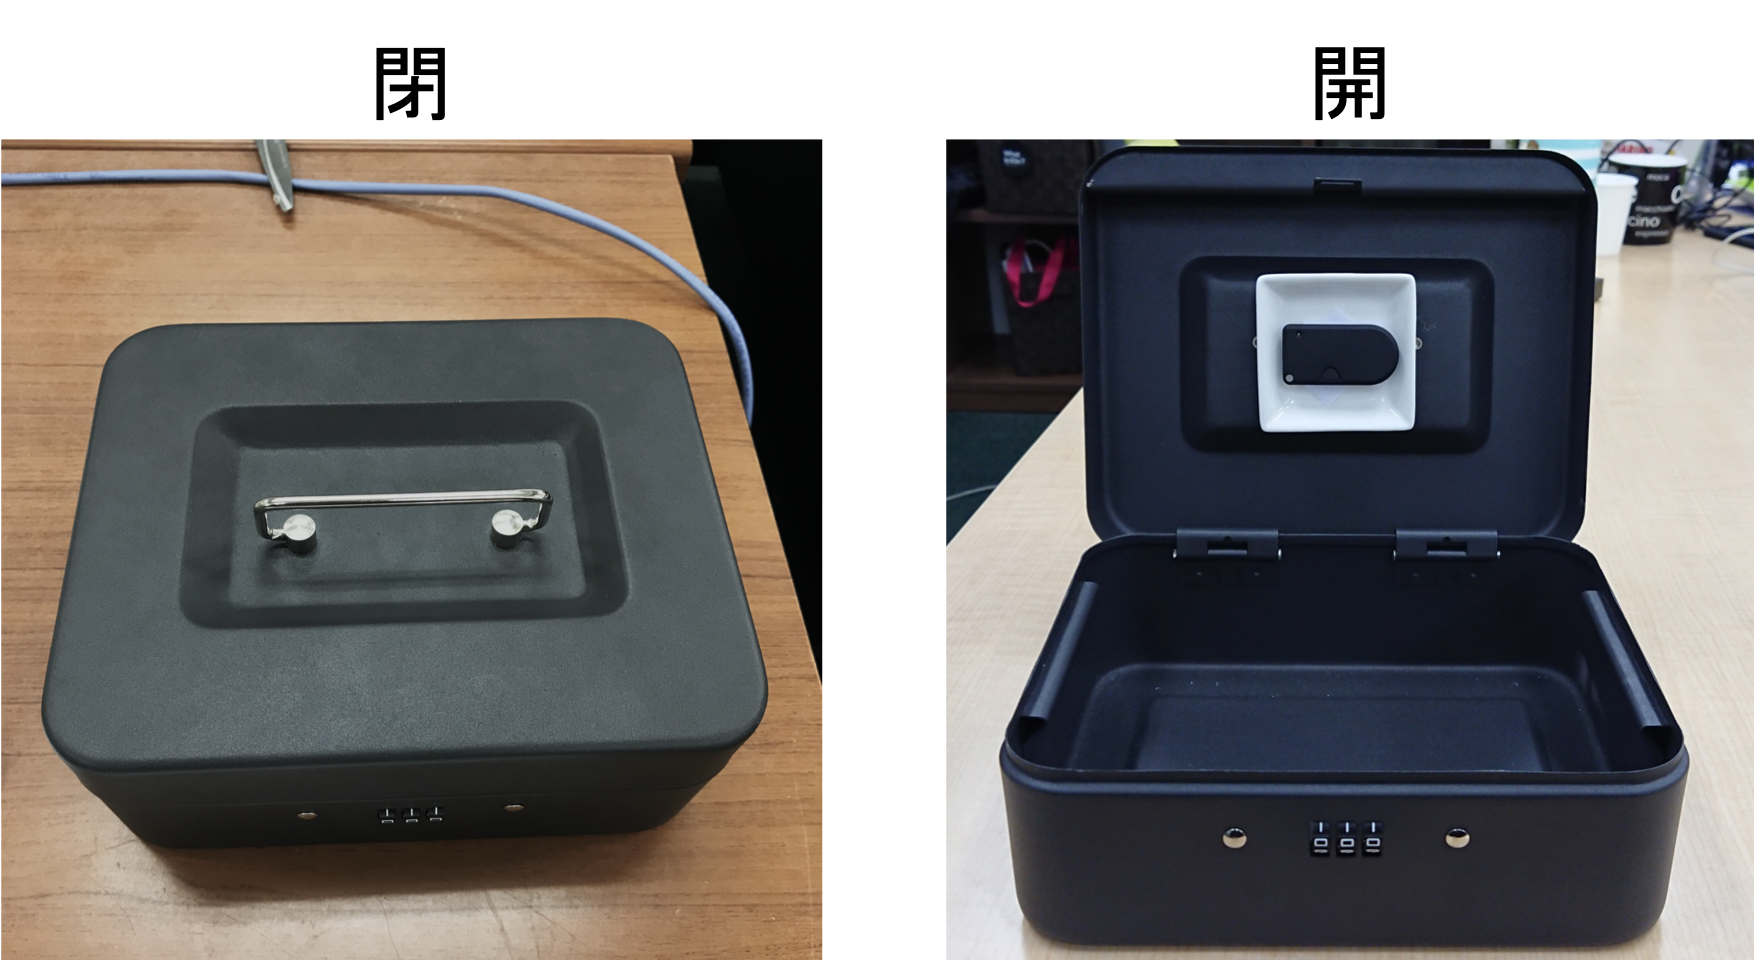
\includegraphics[width=7cm]{kinkoW.png}
    \caption{金庫の状態と設置したビーコン}
    \label{safe}
\end{figure}

\begin{figure}[tbh]
    \centering
    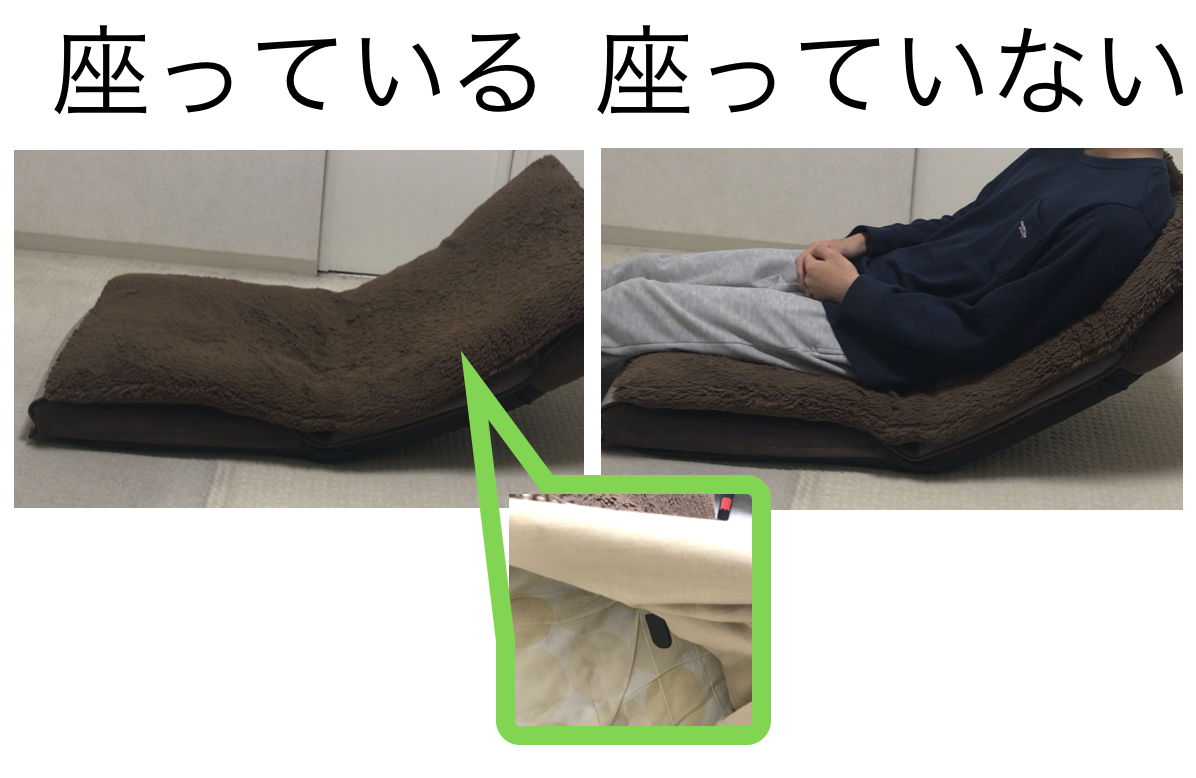
\includegraphics[width=8cm]{zaisuW.png}
    \caption{座椅子の状態と設置したビーコン}
    \label{chair}
\end{figure}




%ーーーーーーーーーーーーーーーーーーーーーーーーーーーーーーーーーーーーーーーーーーーーーーーーー
%ーーーーーーーーーーーーーーーーーーーーーーーーーーーーーーーーーーーーーーーーーーーーーーーーー

\subsection{電波強度のデータ収集対象及び前提}

本研究では受信機としてスマートフォンを使用するため,専用のAndroidアプリケーションを作成し,電波強度の情報を収集する.
その際,BLEビーコンを識別するためのUUID,major,minorをBLEビーコンを設置する対象と紐付けし,どのBLEビーコンの値がどの対象物のモノなのか把握できるようにしている.
また,BLEビーコンの電波送信設定は小さな変化も検知可能にするため送信強度は0dBm,送信間隔は100msと設定した.


%ーーーーーーーーーーーーーーーーーーーーーーーーーーーーーーーーーーーーーーーーーーーーーーーーー
%ーーーーーーーーーーーーーーーーーーーーーーーーーーーーーーーーーーーーーーーーーーーーーーーーー


\subsection{BLEビーコン取り付け位置の検討}
BLEビーコンの取り付け位置や付け方を変えると電波強度の変化に現れる特徴も変えられる.
例えば箱型で蓋の開閉を行う金庫のようなものであれば,BLEビーコンを箱内部の底に設置する場合と蓋の裏に設置する場合が考えられる(図\ref{adapter}).
さらに,対象の材質が電波を通しやすいために状態変化しても電波強度に大きな変化が現れないモノもあるため,図\ref{adapter}のように電波に指向性をもたせるアダプタを取り付け電波強度にはっきりとした変化が出るようにする.
この指向性アダプタとは,図\ref{adapter_only}のような金属や陶器のパラボラアンテナのような形状の物を指し,これを取り付けると電波が拡散せず収束して一方向のみへ飛ぶようになる.
その結果,特定の方向に向かって飛ぶ電波が強まり,状態変化によって電波強度に大きな変化が現れるようになる.

% 図の挿入
\begin{figure}[tbh]
    \centering
    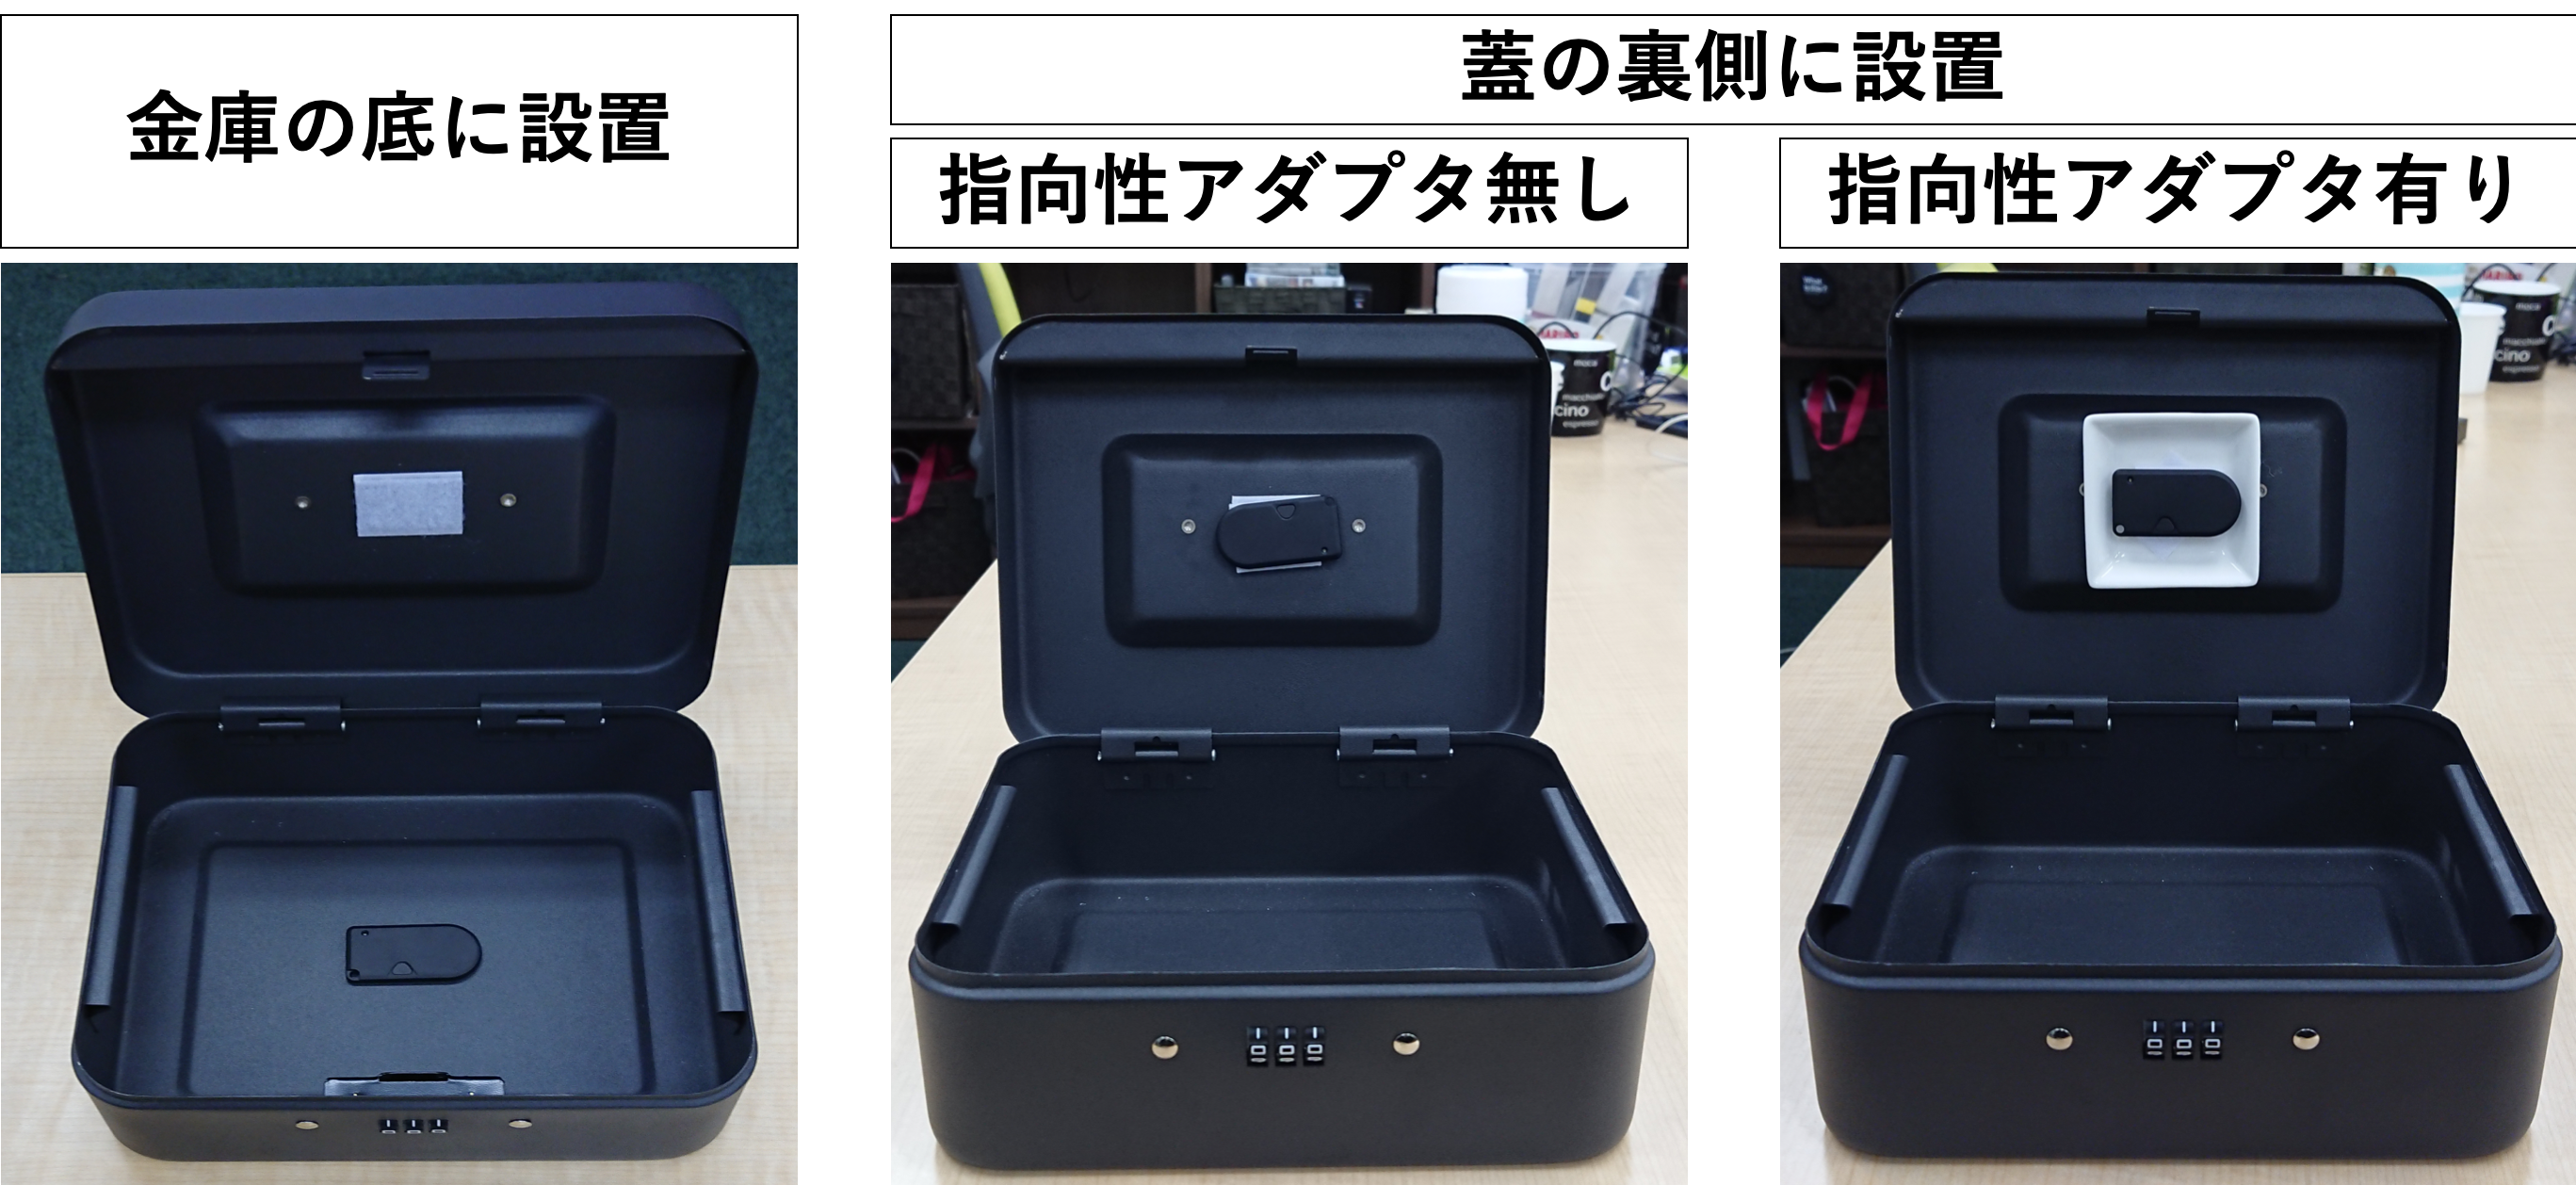
\includegraphics[width=8cm]{adapta_compare2.png}
    \caption{指向性アダプタの有無}
    \label{adapter}
\end{figure}

% 図の挿入
\begin{figure}[tbh]
    \centering
    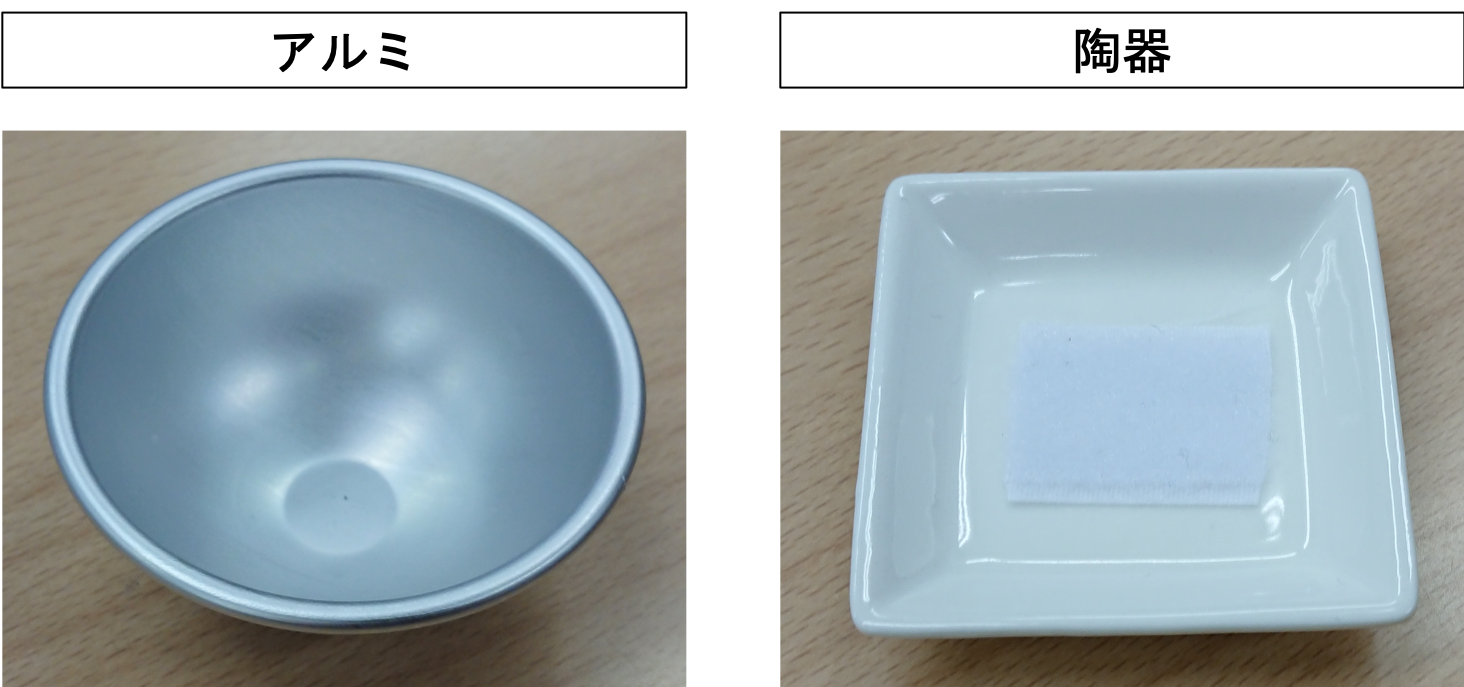
\includegraphics[width=8cm]{adapta.png}
    \caption{本研究で使用した指向性アダプタ}
    \label{adapter_only}
\end{figure}

図\ref{transform-data}にそれぞれの取り付け方による金庫開閉時の電波強度の波形を示す.
この図にはそれぞれ開いている状態と閉じている状態の正解ラベルをつけている.
BLEビーコンを金庫内部の底につけた場合にはあまり大きな変化は見られず,蓋の裏側にBLEビーコンを設置した場合では大きな変化が見られる.
さらに指向性アダプタをつけた場合にはよりくっきりと電波強度に差が現れる.
このようにして状態推定対象それぞれに合わせてBLEビーコンの取り付け方を工夫し,状態変化によって電波強度に大きな変化が現れるようにして状態推定を行う.


% 図の挿入
\begin{figure}[tbh]
    \centering
    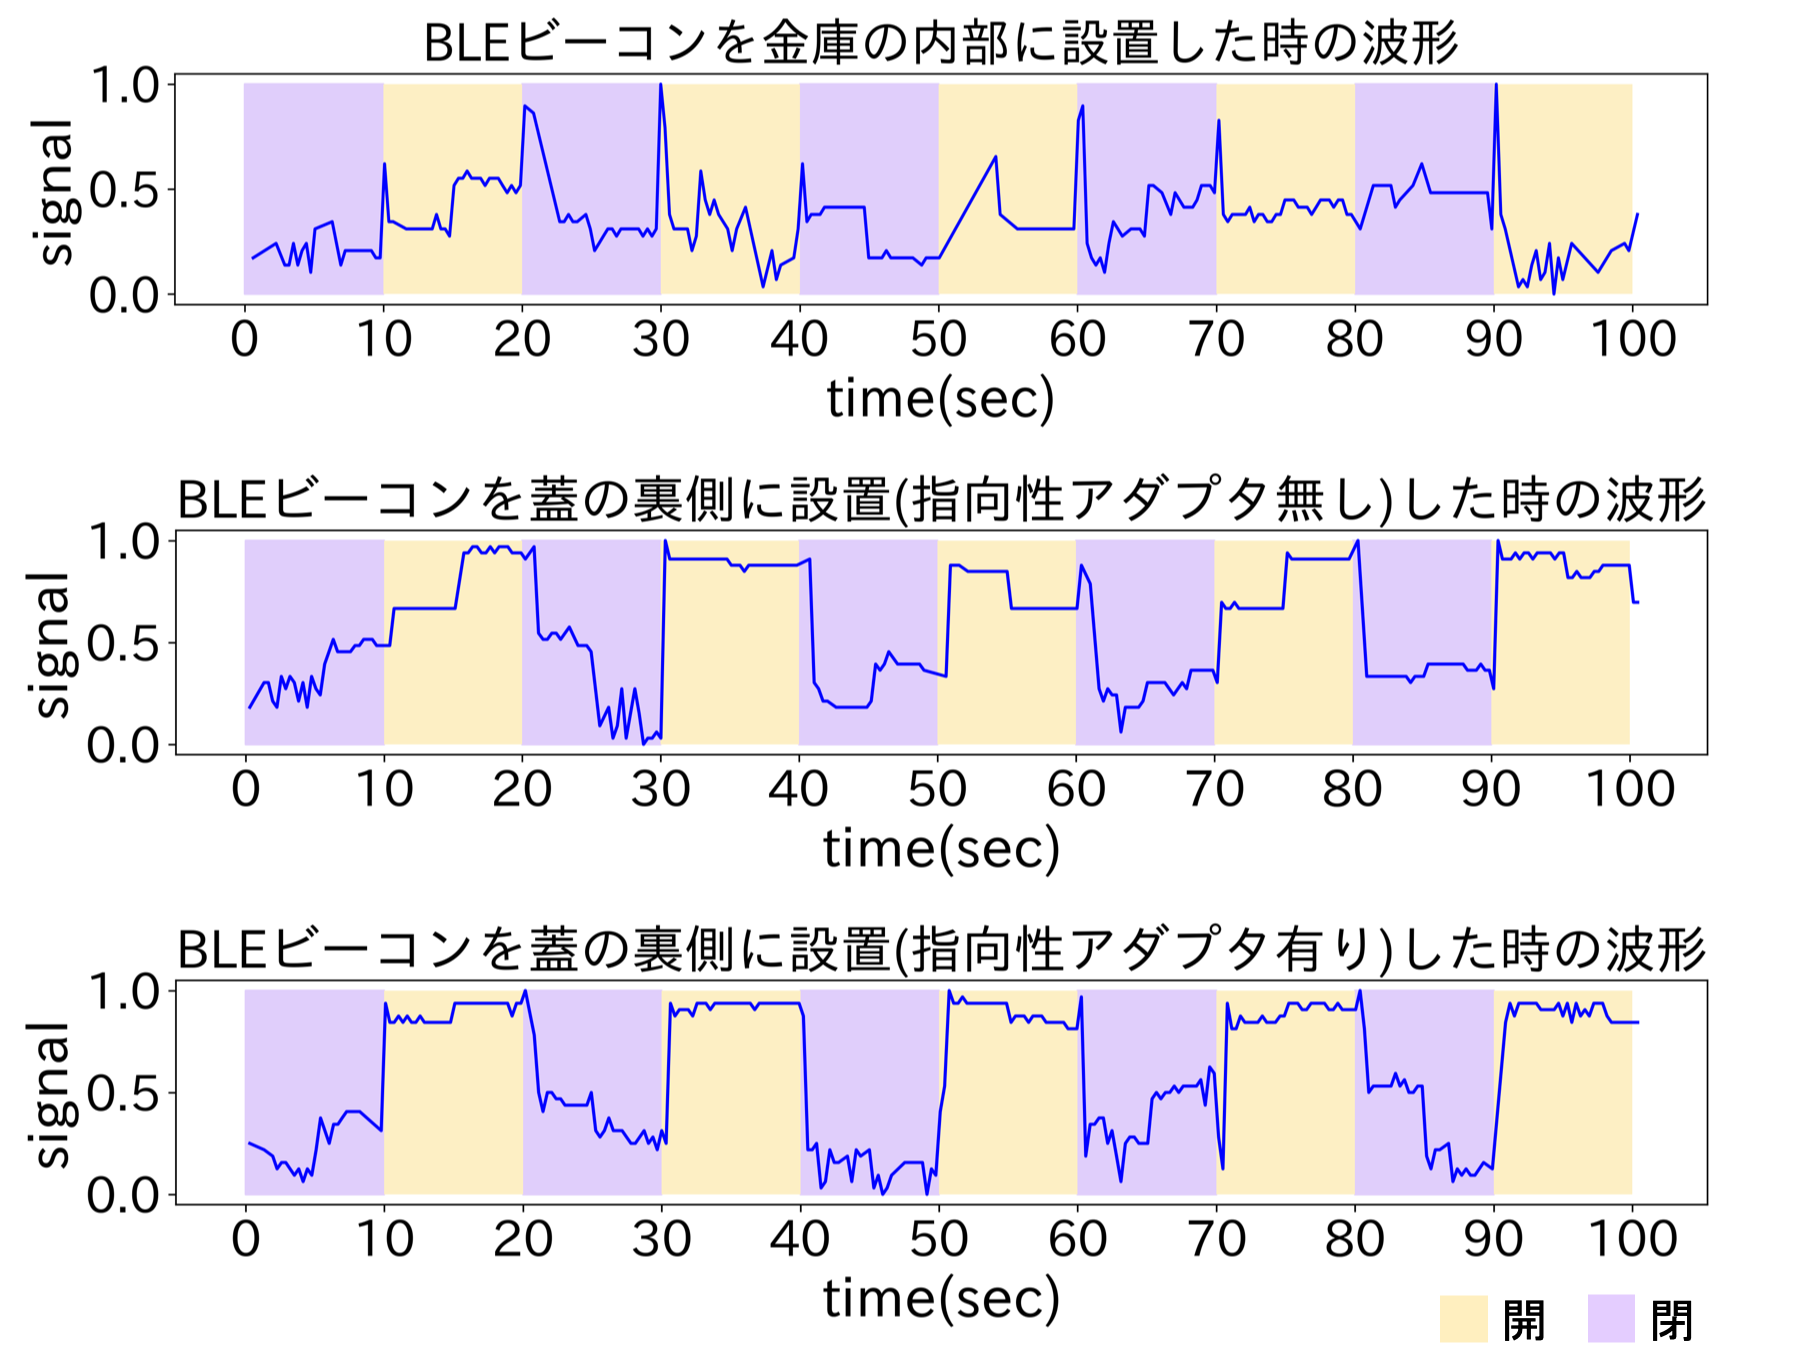
\includegraphics[width=8cm]{in-out.png}
    \caption{ビーコン取り付け位置ごとの電波強度変化}
    \label{transform-data}
\end{figure}


%ーーーーーーーーーーーーーーーーーーーーーーーーーーーーーーーーーーーーーーーーーーーーーーーーー
%ーーーーーーーーーーーーーーーーーーーーーーーーーーーーーーーーーーーーーーーーーーーーーーーーー

\subsection{状態推定アルゴリズム}
本手法ではBLEビーコンから発せられる電波をスマートフォンで300msの間隔で受信し,その受信強度の値から状態を推定する.
図\ref{bank-opcl}は金庫の開閉を行ったときの電波強度の値に,移動平均でローパスフィルタをかけて小さな揺らぎを除去し,値を0から1に正規化したグラフである.
このときローパスフィルタには10個のサンプルつまり3秒分のデータを用いて移動平均を求めている.


\begin{figure}[tbh]
 \centering
 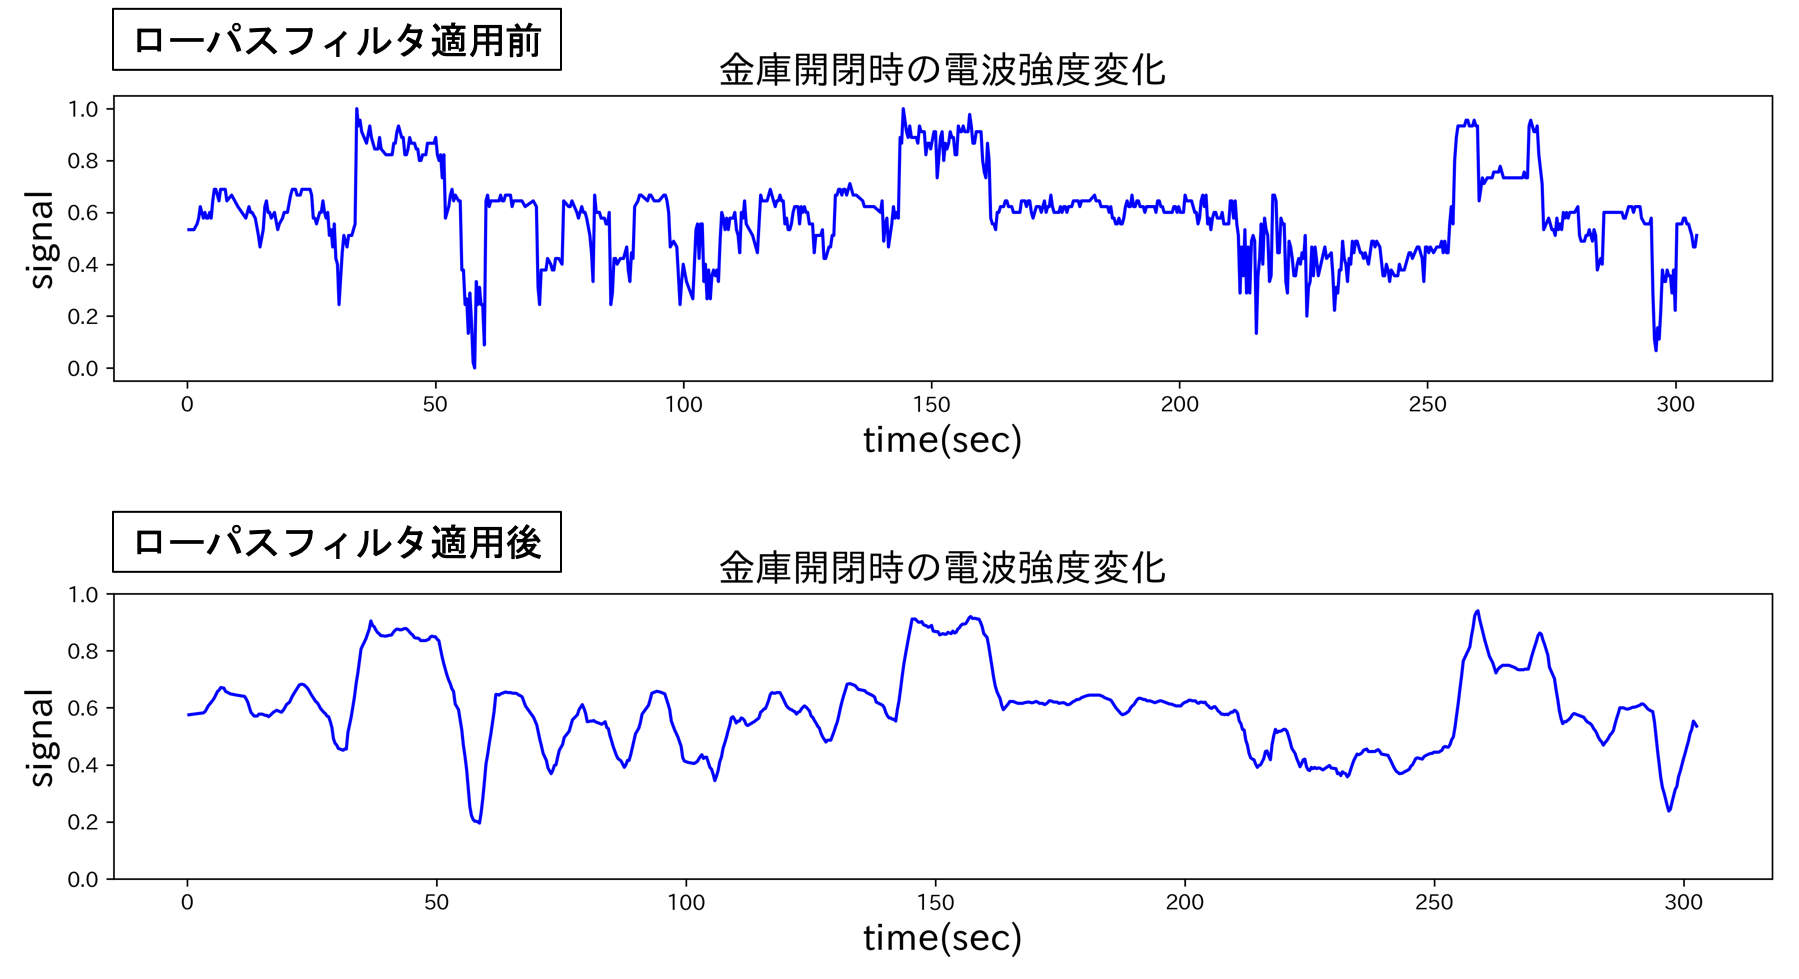
\includegraphics[width=8cm]{lowpath_compare.png}
 \caption{ローパスフィルタ適用前後の電波強度グラフ}
 \label{bank-opcl}
\end{figure}


一時的な障害物があった場合や状態変化に際した人間の影響により電波強度にローパスフィルタでは除去しきれない揺らぎが発生することがあるため,梶ら\cite{sensing-area}が提案している安定センシング区間という概念を利用し推定精度の高精度化を図る.
安定センシング区間とは一定時間以上センシングが安定して行えている区間を指す.
本手法はデータをスマートフォンで収集した後に適用可能なオフライン手法である.


\subsubsection{安定センシング区間}
本手法では推定対象物の移動も考慮するため,安定センシング区間の判定には移動平均を適用したのち閾値を用いて判定を行う.
物体が状態変化をせず移動した場合,電波強度は徐々に変化するため単純な閾値を用いた推定では長距離移動し電波強度が大幅に変化した際に誤判定が起こってしまう.
そこで,取得したすべてのデータから3秒分の移動平均を求め,ある値に着目した際にその値が基準となる値の上限・下限閾値の範囲内であり,かつ一定時間以上経過している場合に安定センシング区間とする.
この時の上限・下限閾値を今回使用したBLEビーコンの特徴や推定対象に合わせ定める.

%@@@@@@@@@@@@@@@@@@@@@@@@@@@@@@@@
図\ref{nomal-data}はBLEビーコンを遮蔽物のない状態で測定した電波強度のグラフであり,ここからBLEビーコンの電波は周期的に電波強度の変化がみられるのが分かる.
このBLEビーコン特有の周期的な電波強度変化により安定センシング区間の判定が不安定になるため,適切な閾値を設定する必要がある.
対象の状態変化による電波強度の変化とBLEビーコン特有の電波強度の変化を考慮して動的に閾値を設定する.


% 図の挿入
\begin{figure}[tbh]
    \centering
    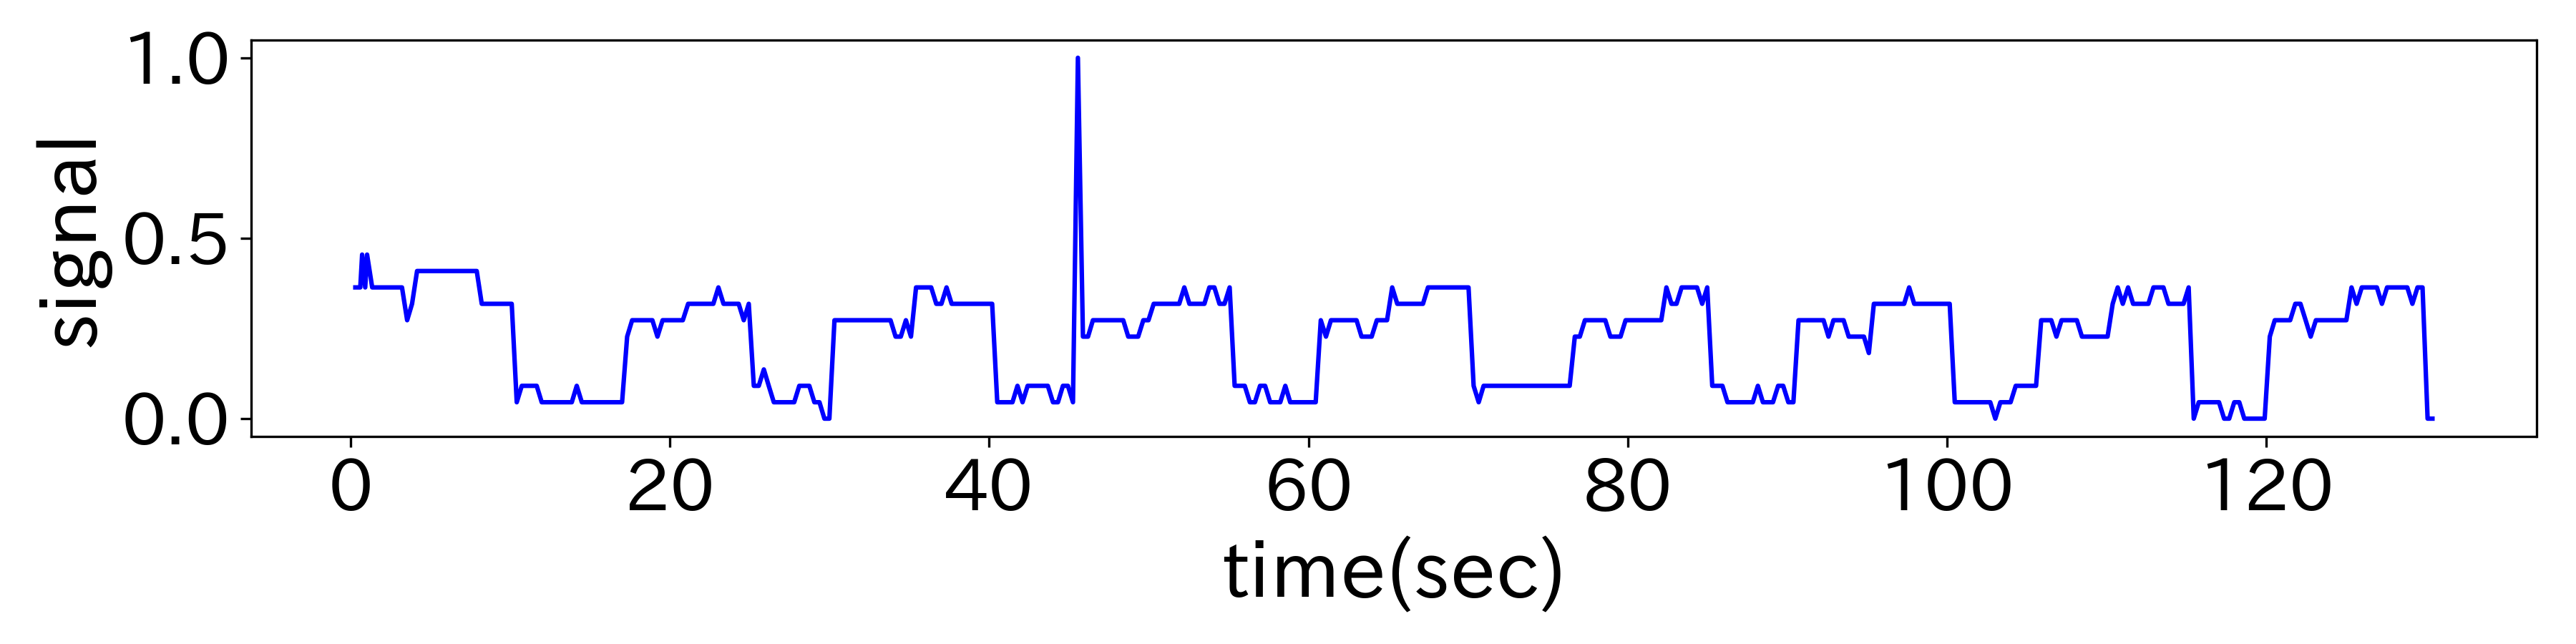
\includegraphics[width=8.5cm]{bokoboko.png}
    \caption{BLEビーコンを遮蔽物のない状態で測定した電波強度グラフ}
    \label{nomal-data}
\end{figure}


%pythonプログラムの説明
オフラインプログラムでは,受信電波強度とその受信時間が記録されたファイルからデータを読み込んで処理を行い状態を推定する.
読み込んだ受信電波強度の数値は0から1の値に正規化し,ローパスフィルタをかけてノイズを取り除く.
次に時系列に並んだデータを走査し,次の値が予め設定しておいた閾値内に受信電波強度の値が収まっているか確認する.
もし閾値を超えた場合は,超える直前の受信電波強度±X(本研究では実験的にX≒0.23として行なっている)の値を新しい閾値として設定する.
これを繰り返し安定センシング区間の判定が終わったら,最後に見つけたそれぞれの安定センシング区間がネガティブな状態かポジティブな状態か判定を行う.


%@@@@@@@@@@@@@@@@@@@@@@@@@@@@@@@@@@



\subsubsection{状態変化の推定}
推定結果の状態をネガティブな状態とポジティブな状態の2つの状態とする.
ポジティブな状態とはBLEビーコンが外に出ていて電波の受信がしやすく、電波強度の値が高い状態を指す. 具体的には金庫の開閉であれば開いてる状態である.
ネガティブな状態とはBLEビーコンが外に出ておらず電波の受信が難しく、電波強度の値が低い状態を指す. 具体的には金庫の開閉であれば閉じてる状態である.
判定は,各安定センシング区間の受信電波強度の平均値が受信電波強度の中央値に0.1を足した値より大きいか小さいかで判定を行う.



%ーーーーーーーーーーーーーーーーーーーーーーーーーーーーーーーーーーーーーーーーーーーーーーーーー
%ーーーーーーーーーーーーーーーーーーーーーーーーーーーーーーーーーーーーーーーーーーーーーーーーー


\section{評価実験}

本稿で提案した手法の推定精度を確かめるため,いくつかのモノへBLEビーコンを設置し評価実験を行った.
BLEビーコンを設置する対象は,冷蔵庫,金庫,座椅子とし,金庫と座椅子については移動を考慮した状態変化に対し推定精度を測定した.
評価の方法は開閉などの状態変化をランダムな間隔で行い,その推定結果と正解ラベルを比べて正答率を算出して行った.

\subsection{実験端末の選定}

\begin{figure}[tbh]
    \centering
    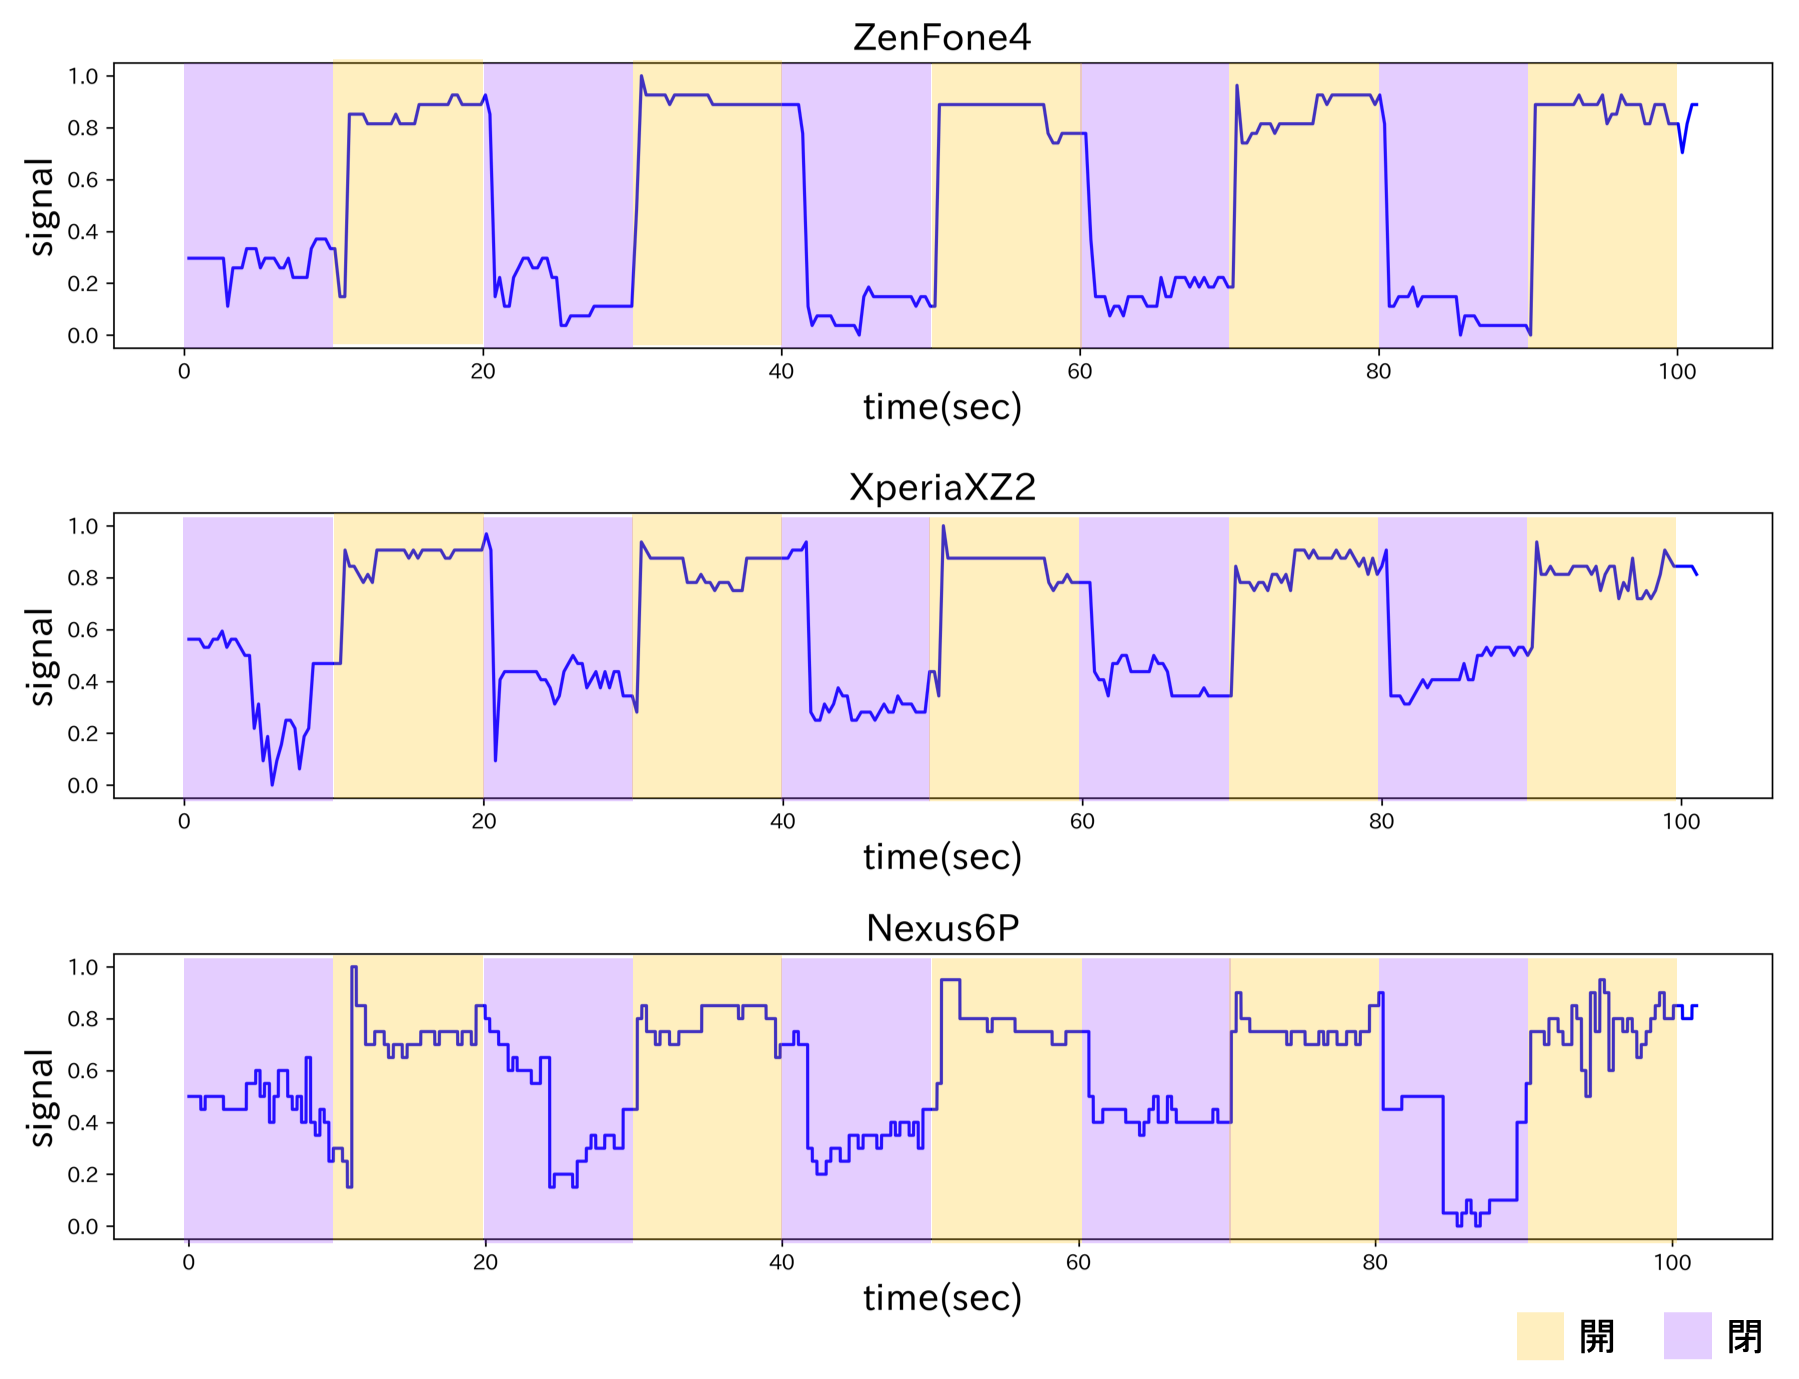
\includegraphics[width=8cm]{mix.png}
    \caption{機種ごとの精度比較}
    \label{multi-data}
\end{figure}

Bluetoothのセンサ精度は端末ごとに異なるため,実験に用いる端末は変化を正しく捉えられる端末を使うのが望ましい.
そこでAndroid端末を3機種用意し,同一環境下で金庫の蓋の開閉を行い測定精度の比較を行った.
今回用意した端末はXperia XZ2,Nexus 6P,ZenFone 4である.
金庫開閉時の電波強度変化を各端末で収集し,その波形を比較した結果を図\ref{multi-data}に示す.
図の紫色の部分は蓋が閉まっている状態を黄色の部分は蓋が開いている状態を示している.
3機種の精度を比較した結果,Nexus 6Pでは全体的に小さなノイズが発生しているがZenFone 4とXperia XZ2ではそれが少ない.
また,Xperia XZ2とNexus 6Pは測定開始直後は測定値が安定せず正しく変化を捉えられていない.

本手法では電波強度の急激な変化と安定センシング区間の判定が重要となるため,測定ノイズが少なく電波を正確に捉えられる必要がある.
そのためこの3機種のうち一番ノイズが少なく,正解ラベルと比べもっともらしい値を捉えられるZenFone 4を実験で用いる受信機として使用した.
また,本研究では金庫などの移動を伴う比較的小さなモノにもBLEビーコンを取り付けるため,使用するBLEビーコンはできるだけ小さい方が望ましい.
そのためBLEビーコンは軽量・小型という理由からフォーカスシステムズ社のFCS1301\ref{beacon}を使用した.


\subsection{冷蔵庫の開閉における推定精度の測定}
図\ref{freezer},図\ref{refrigerator_position}のようにBLEビーコンを設置した冷蔵庫と受信機を設置して評価実験を行った.
実験は日常の使用を模倣し,冷蔵庫のドアを開けて,中からペットボトルを取り出し,ドアを閉めるという動作をランダムな間隔で行い,その状態変化を捉えられるか評価を行った.
%@@@@@@@@@@@@@@@@@@@@@@@@
%時間と閾値の話をして


\begin{figure}[tbh]
    \centering
    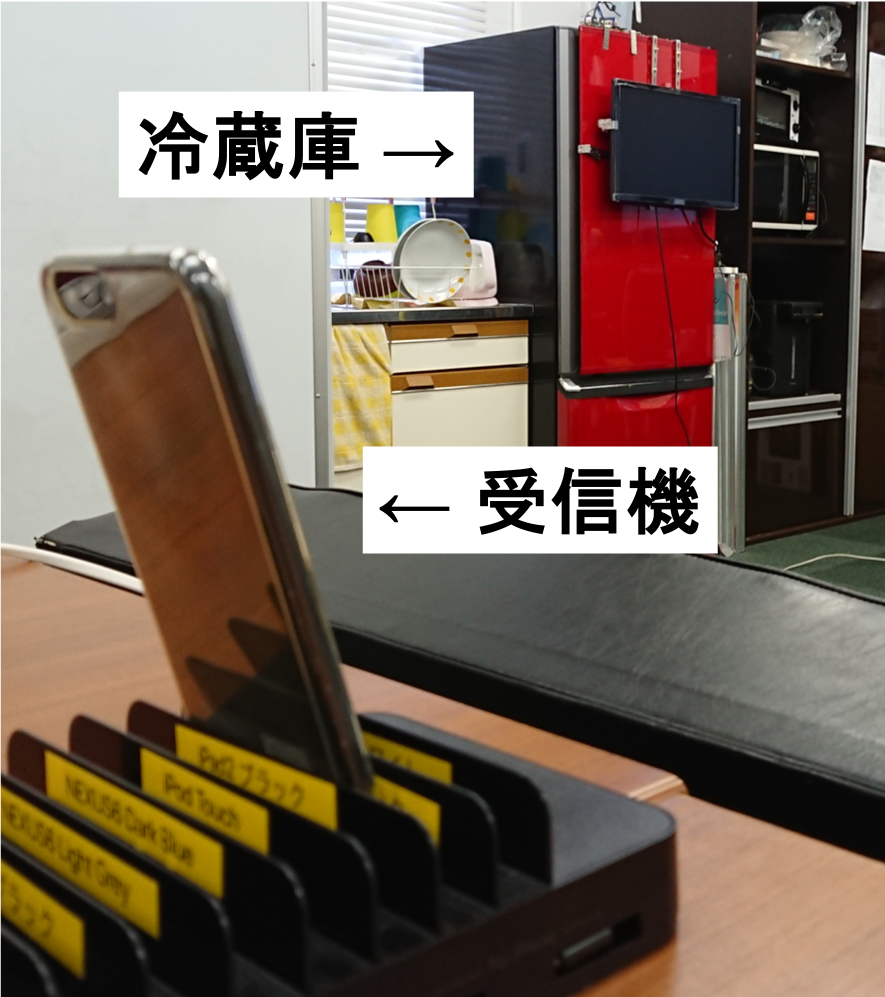
\includegraphics[width=8cm]{refrigerator_position.png}
    \caption{冷蔵庫と受信機の位置関係図}
    \label{refrigerator_position}
\end{figure}


日常使いにおいて冷蔵庫を開ける動作時間は約7秒程度であるため本実験でもそれを模倣し,閉めている状態はランダムに1分から5分程度の時間を設けた.
この時,冷蔵庫が開いている状態も推定可能にするため安定センシング区間を判定する閾値はそれぞれ,値の閾値を±0.23,時間の閾値を2秒に設定した.
%@@@@@@@@@@@@@@@@@@@@@
BLEビーコンを扉の棚へ置いただけではあまり電波強度に変化が見られなかったため,電波強度の変化を大きくさせるよう3.2章で述べた指向性アダプタを取り付けた.
推定結果を図\ref{refrigerator_graph}に,正解率の一覧を表\ref{refrigerator_fig}に示す.
図\ref{refrigerator_graph}の白色の範囲は安定センシング区間ではない状態を 緑色の範囲はネガティブな状態(ドアが閉まっている状態)を 赤色の範囲はポジティブな状態(ドアが開いている状態)を示している.
%また,表\ref{refrigerator_fig}には各試行における正解率とその累計正解率,及び正推定ラベルのうち正しく推定できた時間の割合を示している.

同様の実験を3回行った結果1回だけ不正解があり,試行回数をもとにした状態推定精度は98.0%,推定ラベルのうち正しく推定できた時間をもとにした状態推定精度は99.2%となった.
% 誤判定された400秒付近のグラフを見てみると他と比べて受信電波強度の変化が小さく,安定センシング区間と判定されていない.


\begin{figure}[tbh]
    \centering
    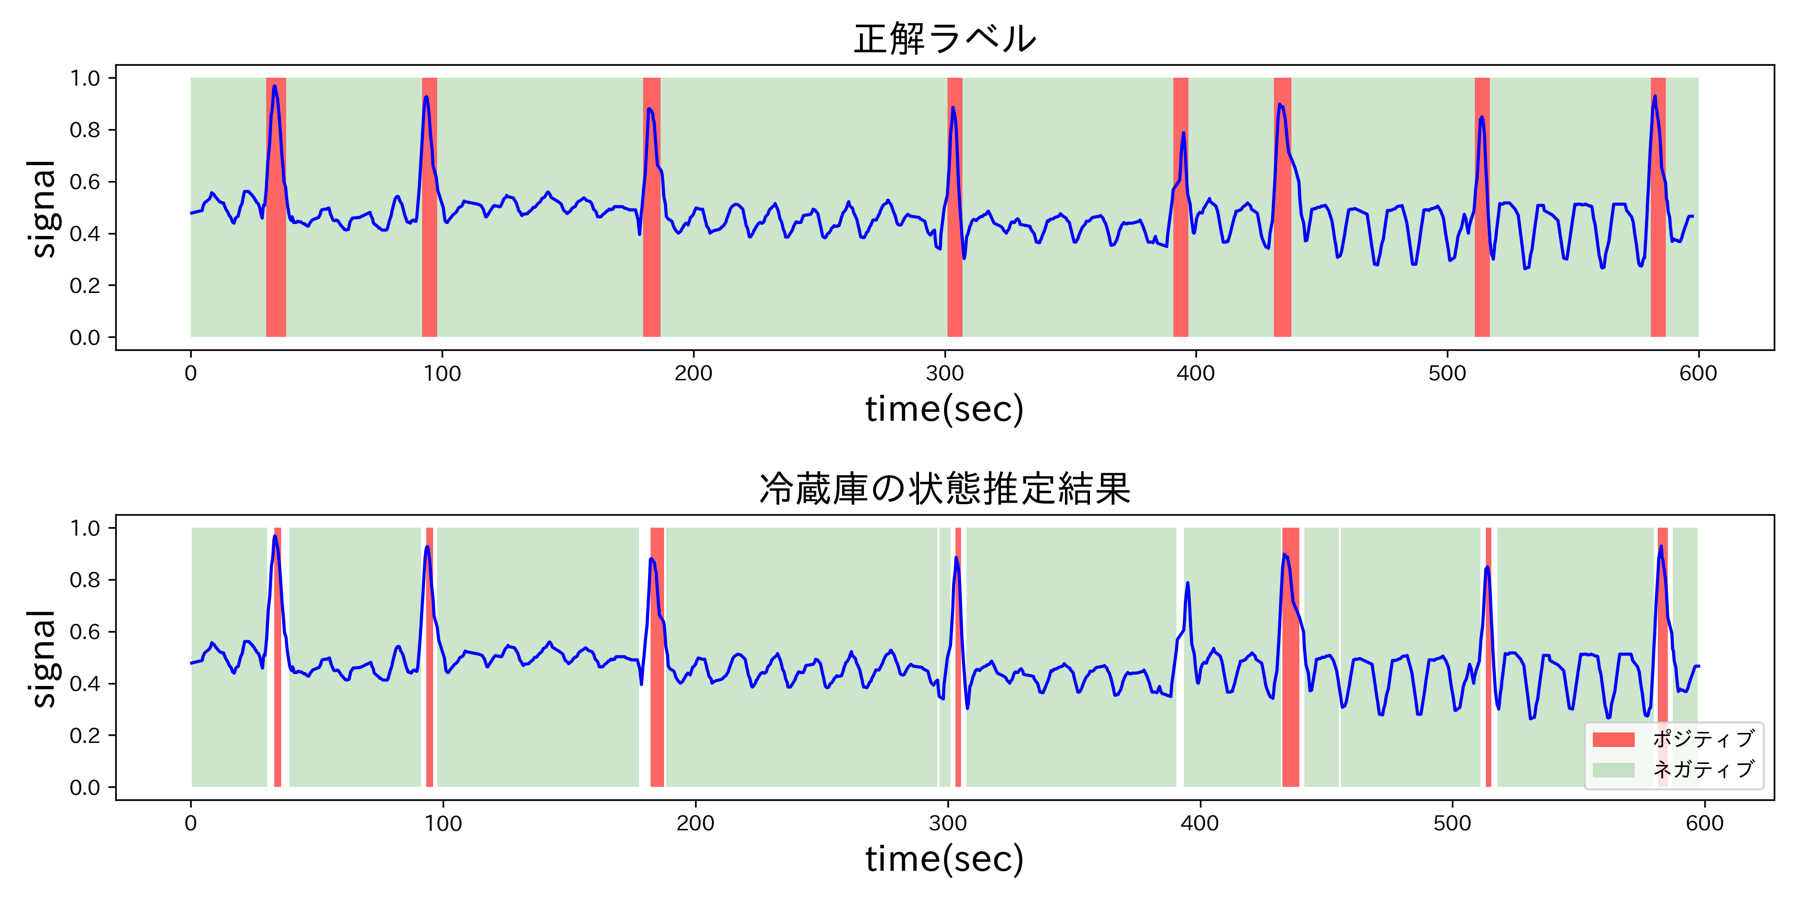
\includegraphics[width=8cm]{refrigerator_graph.png}
    \caption{冷蔵庫の状態推定結果グラフ}
    \label{refrigerator_graph}
\end{figure}


%@@@@@@@@@@@@@@@@@@@@
%  ポジティブな状態だけ検出できた割合の結果 ではなくネガティブポジティブ両方の検出数から割合を出すべきでは????
%@@@@@@@@@@@@@@@@@@@@
\begin{table}[tbh]
    \begin{center}
        \caption{冷蔵庫の開閉における状態推定精度}
        \label{refrigerator_fig}
        \begin{tabular}{|c|c|c|c|} \hline
        試行回数 & 正答率 & 正解数 & 不正解数 \\ \hline
        1 & 94.1% & 16 & 1 \\ \hline
        2 & 100% & 17 & 0 \\ \hline
        2 & 100% & 17 & 0 \\ \hline \hline
        回数でみた累計正解率 & \multicolumn{3}{c|}{98.0%} \\ \hline \hline
        推定ラベルの正解割合 & \multicolumn{3}{c|}{99.2%} \\ \hline
        \end{tabular}
    \end{center}
\end{table}



\subsection{金庫の開閉における推定精度の測定}
図\ref{safe},図\ref{kinko_position}のようにBLEビーコンを設置した金庫と受信機を設置して評価実験を行った.
金庫は図\ref{kinko_position}のようにまず1の場所で開閉を行い,2の場所へ移動させたのち開閉を行い最後に3の場所に移動させたのち開閉を行い,推定中にモノの移動が行われても状態推定が可能かを確かめた.
この時,金庫を開けている時間は約20秒程度であり,閉めた状態はランダムに30秒から2分程度継続させた.
また,安定センシング区間を判定する閾値はそれぞれ,値の閾値を±0.23,時間の閾値を4.5秒に設定した.
%@@@@@@@@@@@@@@@@@@@@@@@
%閾値の話して
%ちゃんとなんでかの理由も含めれると良いけど
%@@@@@@@@@@@@@@@@@@@@@@@

推定結果を図\ref{kinko_graph}に,正解率の一覧を表\ref{kinko_fig}に示す.
図\ref{kinko_graph}の白色の範囲は安定センシング区間ではない状態を 緑色の範囲はネガティブな状態(蓋が閉まっている状態)を 赤色の範囲はポジティブな状態(蓋が開いている状態)を示しており,図中の番号は図\ref{kinko_position}内の番号と対応している.
%また,表\ref{kinko_fig}には各試行における正解率とその累計正解率,及び正推定ラベルのうち正しく推定できた時間の割合を示している.

同様の実験を3回行った結果,試行回数をもとにした状態推定精度は100%,推定ラベルのうち正しく推定できた時間をもとにした状態推定精度は93.8%であった.
% 正解ラベル通りの推定ができていなかった2番の場所での推定結果を見ると,蓋が閉まった後も数秒間蓋が開いていると推定されてしまっている.

\begin{figure}[tbh]
    \centering
    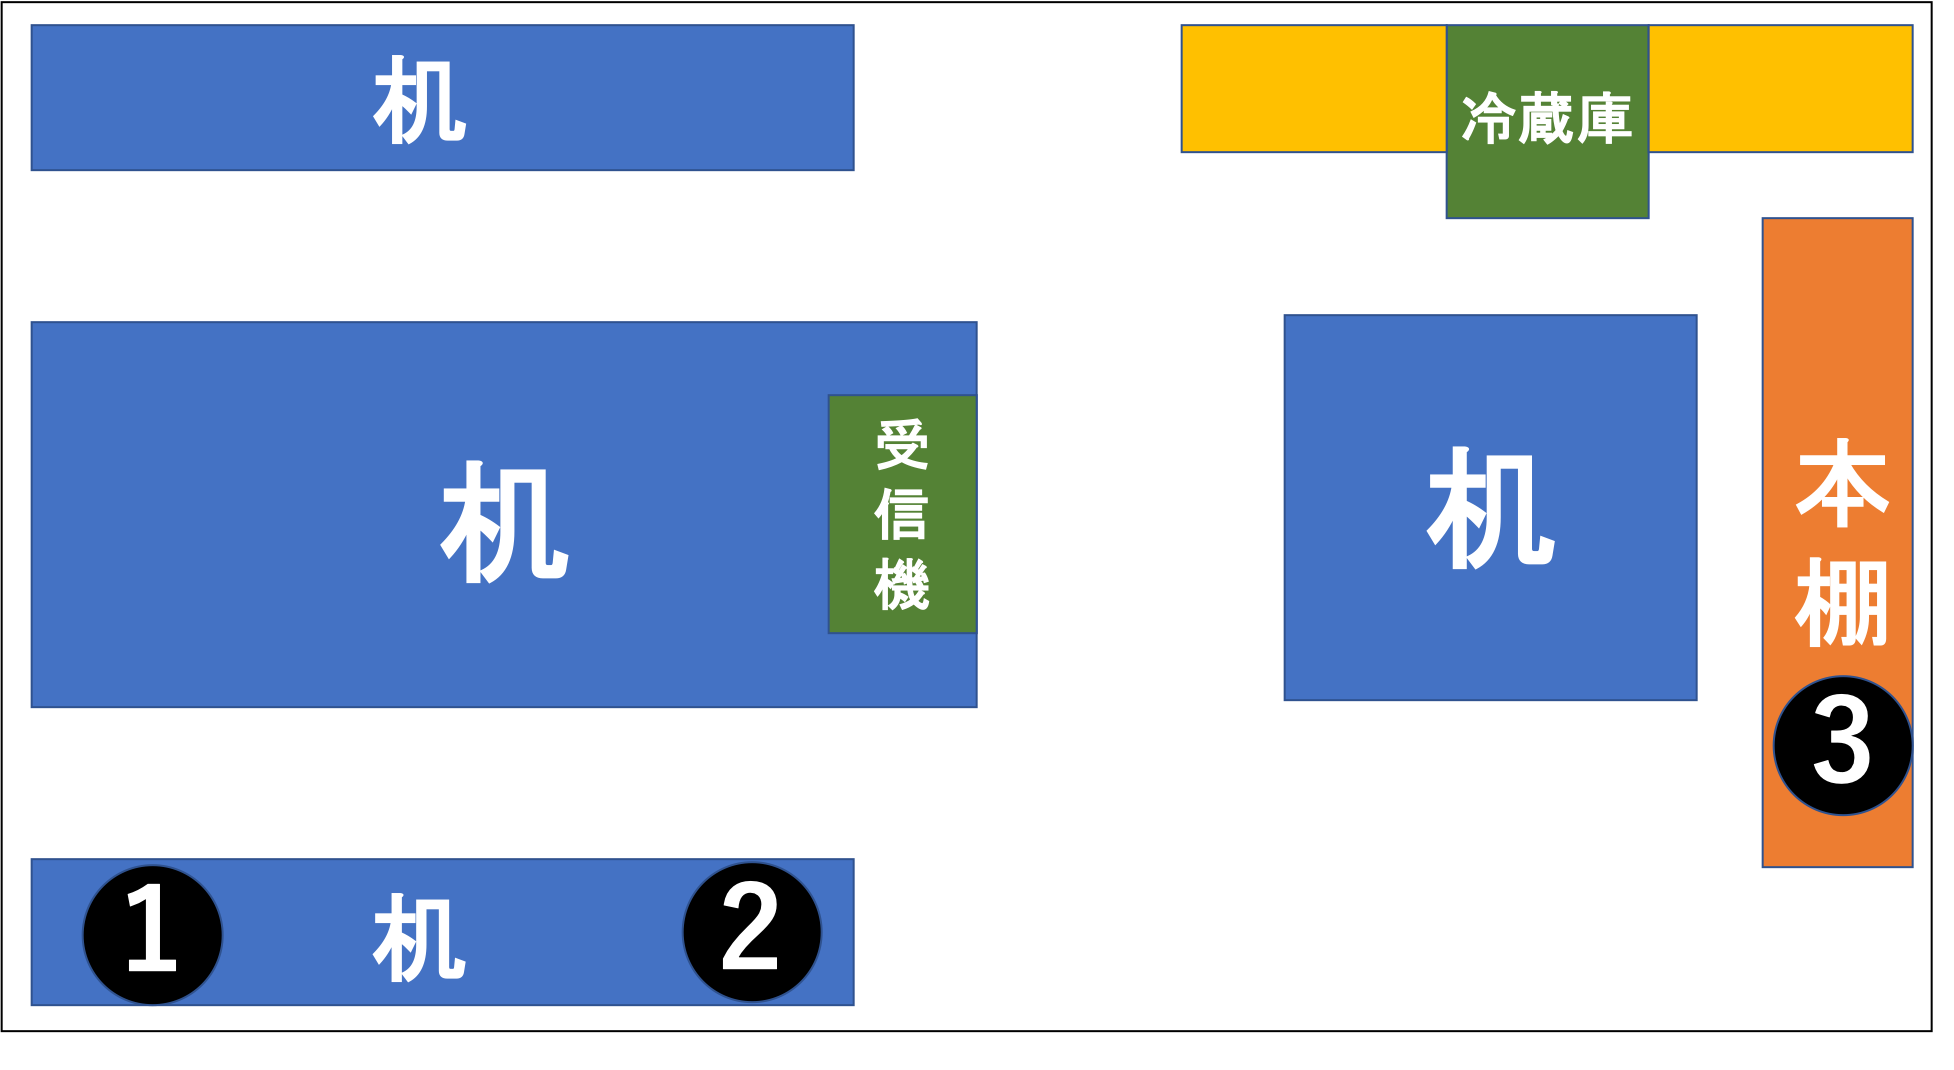
\includegraphics[width=8cm]{kinko_position_fig.png}
    \caption{金庫と受信機の位置関係図}
    \label{kinko_position}
\end{figure}

\begin{figure}[tbh]
    \centering
    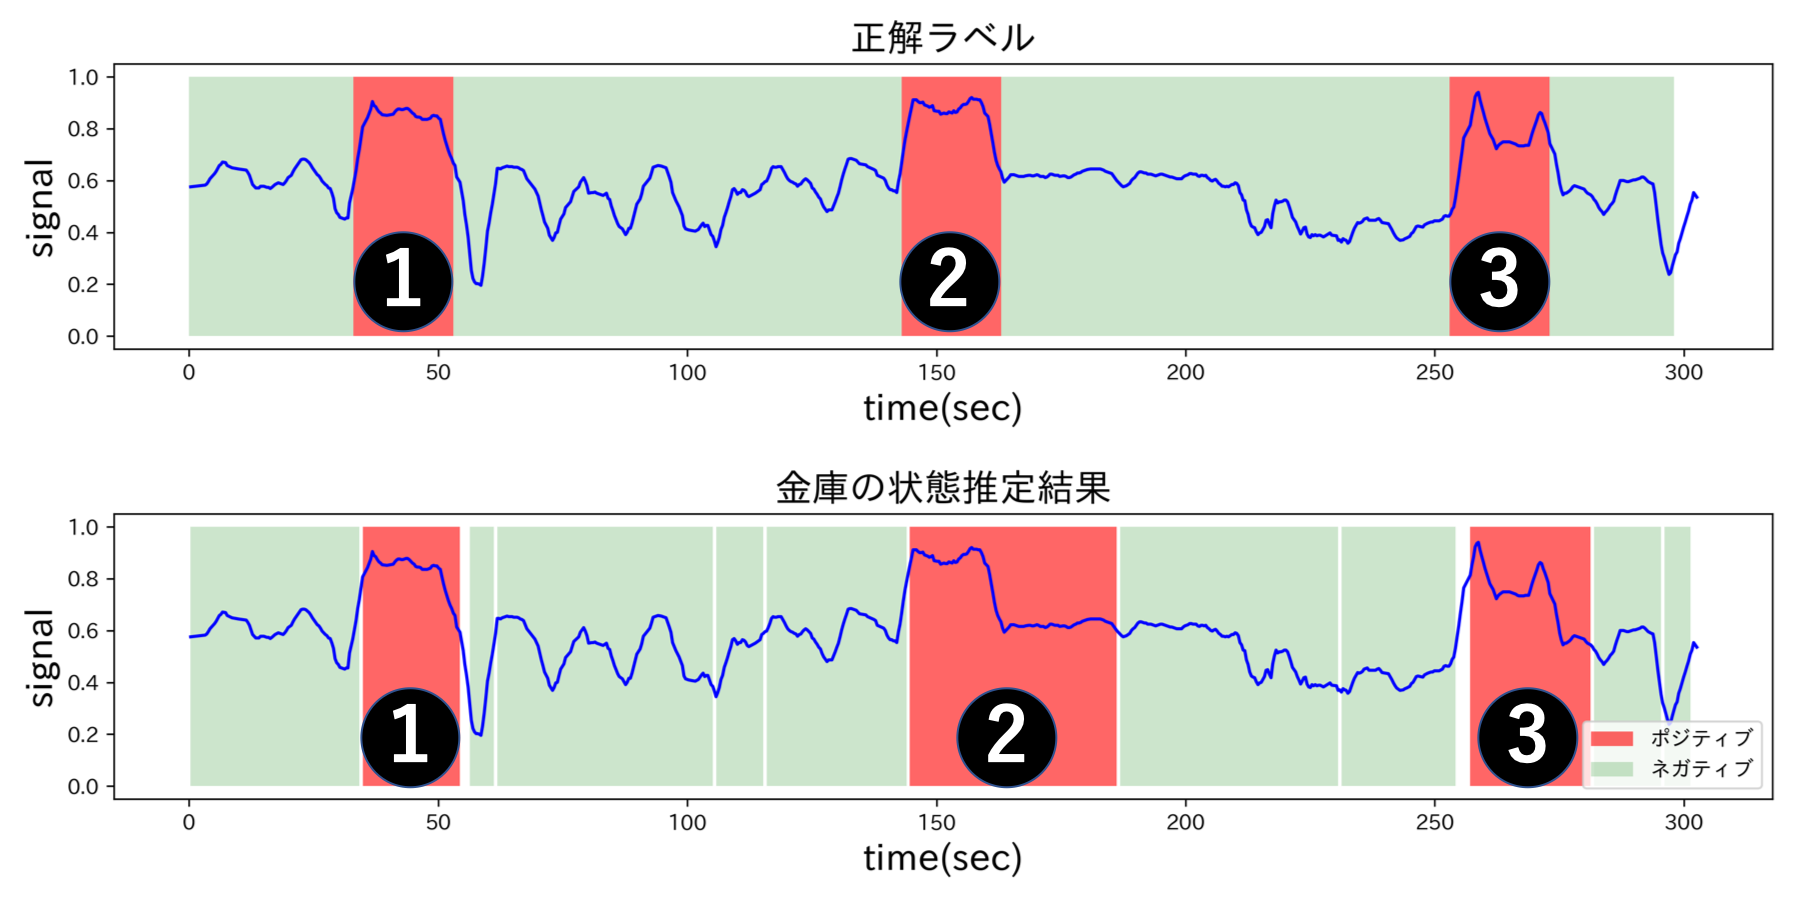
\includegraphics[width=8cm]{kinko_graph.png}
    \caption{金庫の状態推定結果グラフ}
    \label{kinko_graph}
\end{figure}

\begin{table}[tbh]
    \begin{center}
        \caption{金庫の開閉における状態推定精度}
        \label{kinko_fig}
        \begin{tabular}{|c|c|c|c|} \hline
        試行回数 & 正答率 & 正解数 & 不正解数 \\ \hline
        1 & 100% & 7 & 0 \\ \hline
        2 & 100% & 7 & 0 \\ \hline
        2 & 100% & 7 & 0 \\ \hline \hline
        回数でみた累計正解率 & \multicolumn{3}{c|}{100%} \\ \hline \hline
        推定ラベルの正解割合 & \multicolumn{3}{c|}{93.8%} \\ \hline

        \end{tabular}
    \end{center}
\end{table}



\subsection{座椅子の着座における推定精度の測定}

%@@@@@@@@@@@@@@@
%使用したパラメータ
%filter_size = 10      # ローパスフィルタのフィルターサイズ
%sz_interval = 5       # 安定センシング区間を判断する時間間隔
%sz_under = 0.235      # 安定センシング区間だと判断する閾値の下限
%sz_upper = 0.235      # 安定センシング区間だと判断する閾値の上限
%@@@@@@@@@@@@@@@
図\ref{chair},図\ref{zaisu_position}のようにBLEビーコンを設置した座椅子と受信機を設置して評価実験を行った.
動作の流れとして,1の位置で着座を行ったのち2の場所に移動させ着座を行った.
座椅子に座っている時間として30秒から1分30秒程度を,座っていない時間として30秒から2分程度を設定した.
推定結果を図\ref{chair_graph}に,正解率の一覧を表\ref{chair_fig}に示す.
この時安定センシング区間を判定のための閾値はそれぞれ,値の閾値は±0.235,時間の閾値は5秒に設定した.


\begin{figure}[tbh]
    \centering
    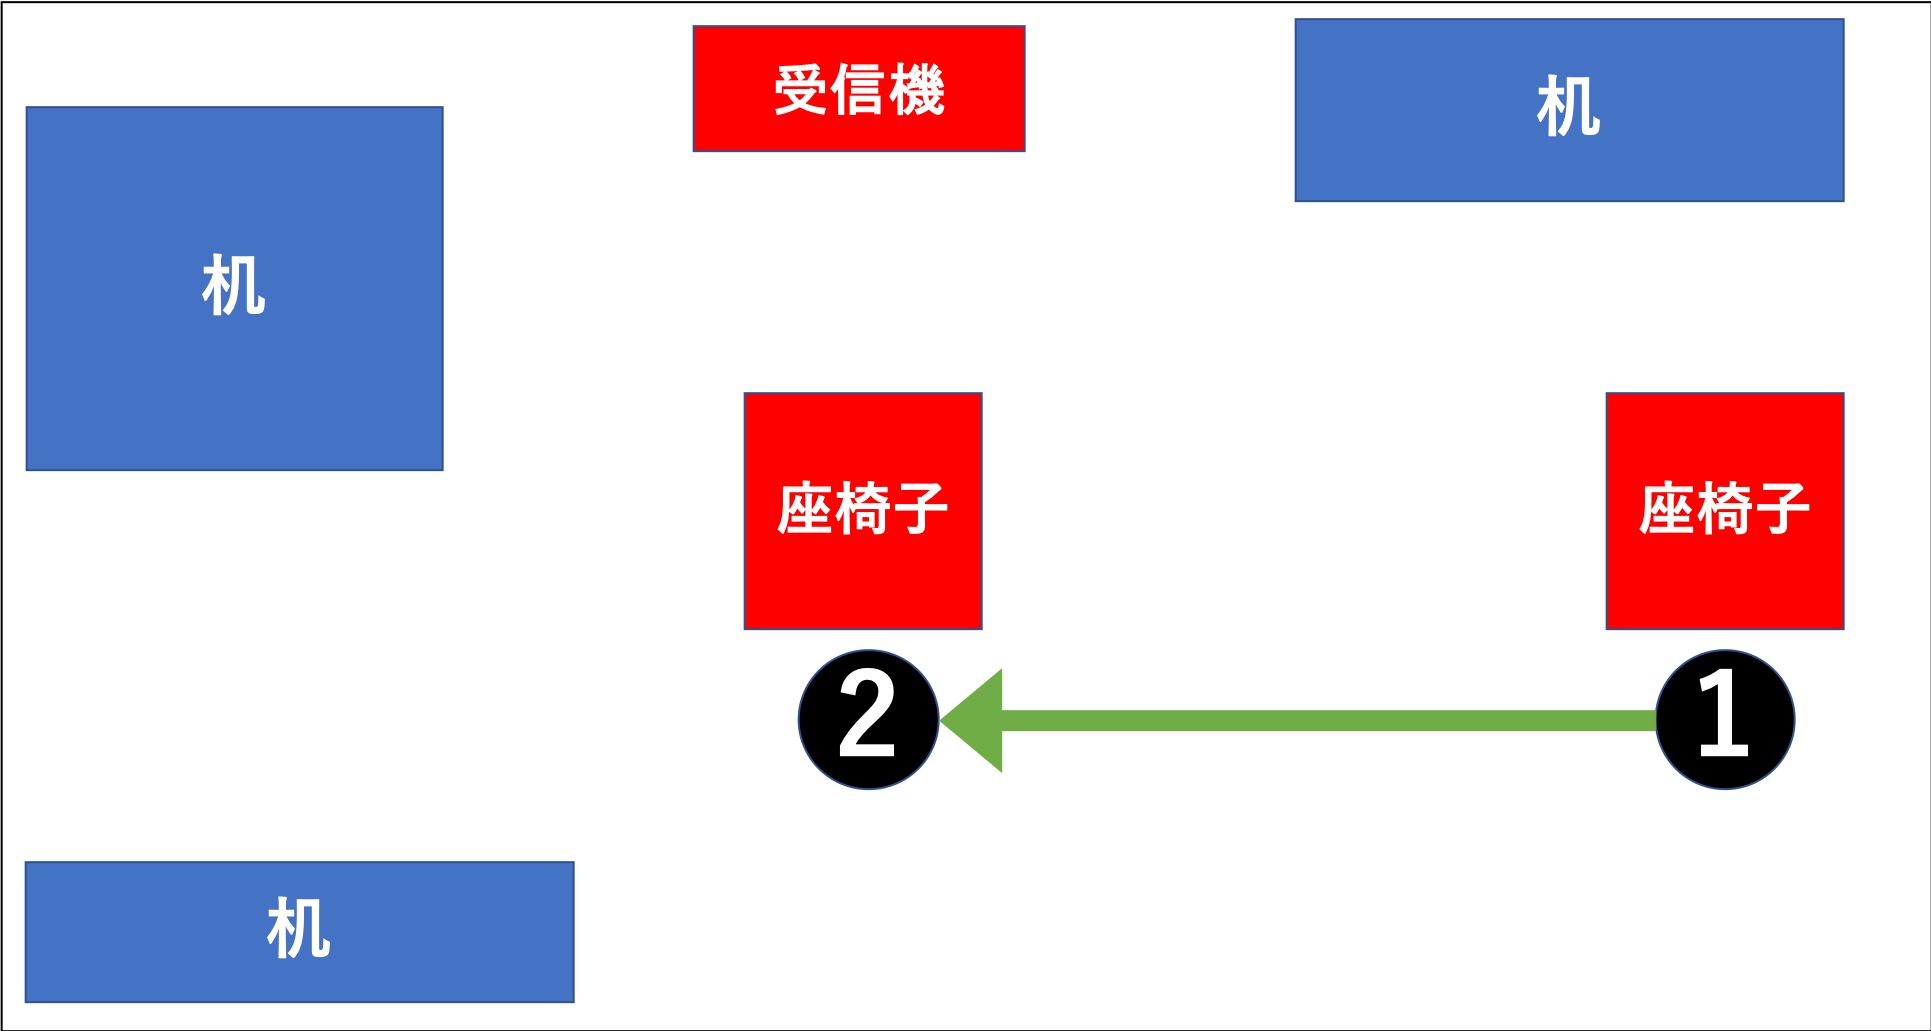
\includegraphics[width=8cm]{zaisu_position.png}
    \caption{座椅子と受信機の位置関係図}
    \label{zaisu_position}
\end{figure}


\begin{figure}[tbh]
    \centering
    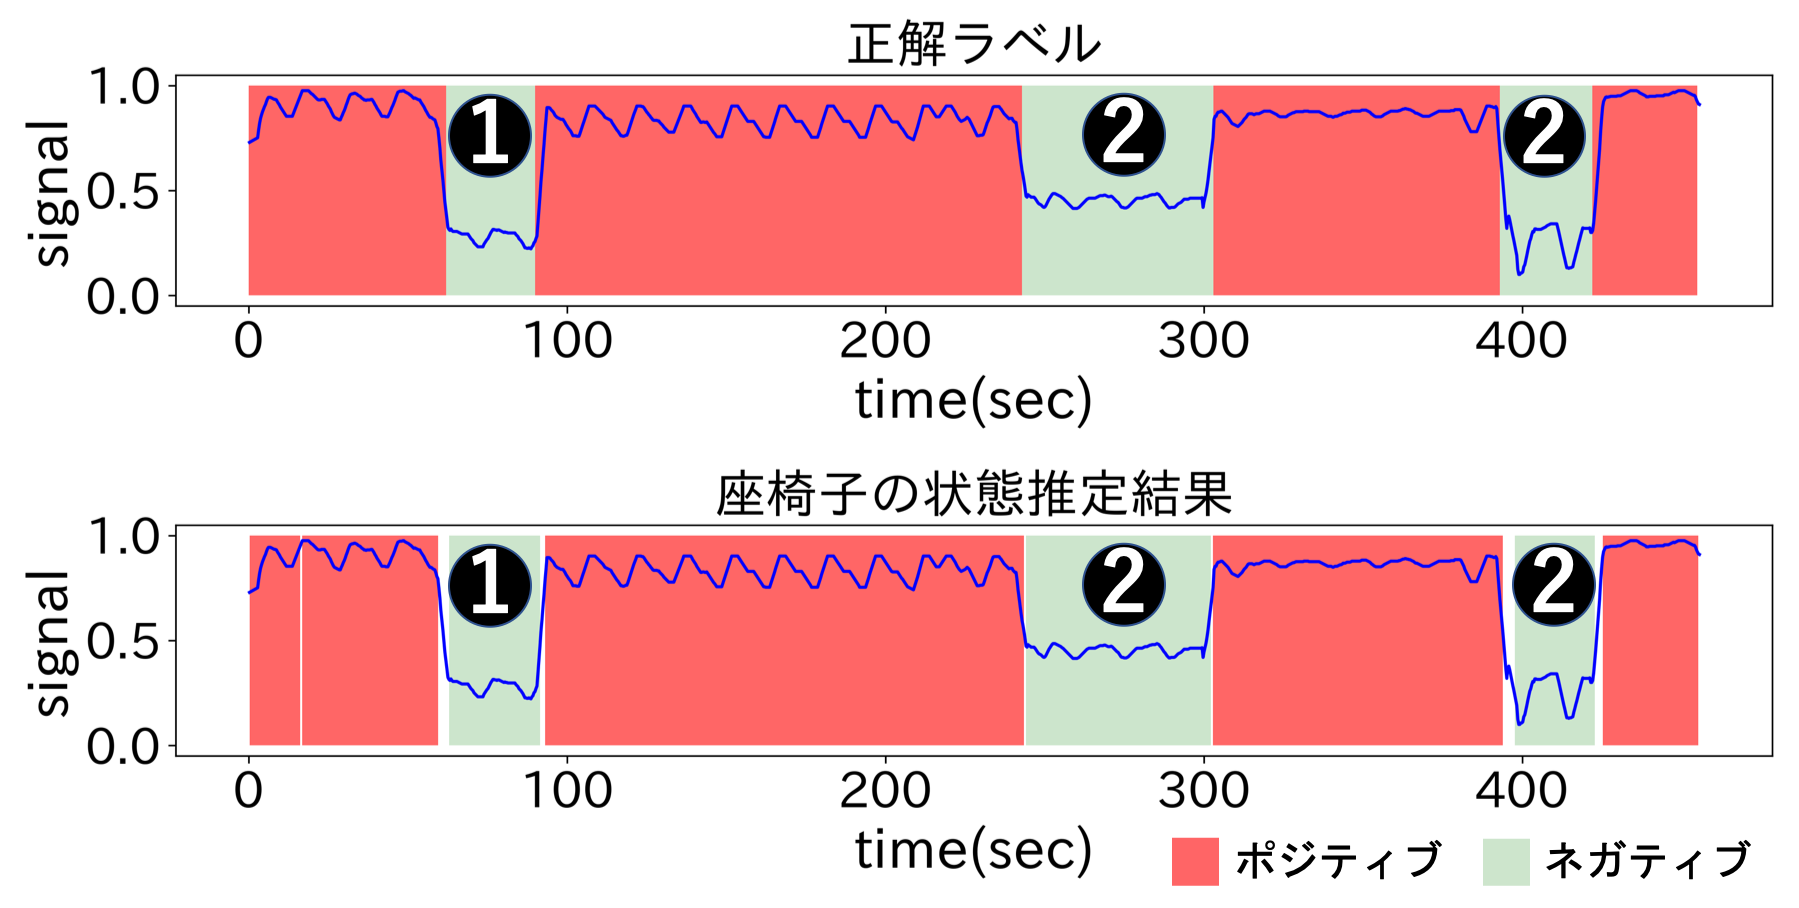
\includegraphics[width=8cm]{zaisu_graph.png}
    \caption{座椅子の状態推定結果グラフ}
    \label{chair_graph}
\end{figure}


\begin{table}[tbh]
    \begin{center}
        \caption{座椅子への着席における状態推定精度}
        \label{chair_fig}
        \begin{tabular}{|c|c|c|c|} \hline
        試行回数 & 正答率 & 正解数 & 不正解数 \\ \hline
        1 & 100% & 7 & 0 \\ \hline
        2 & 100% & 7 & 0 \\ \hline
        2 & 100% & 7 & 0 \\ \hline \hline
        回数でみた累計正解率 & \multicolumn{3}{c|}{100%} \\ \hline \hline
        推定ラベルの正解割合 & \multicolumn{3}{c|}{98.9%} \\ \hline

        \end{tabular}
    \end{center}
\end{table}


図\ref{chair_graph}の白色の範囲は安定センシング区間ではない状態を 緑色の範囲はネガティブな状態(人が座っている状態)を 赤色の範囲はポジティブな状態(人が座っていない状態)を示しており,図中の番号は図\ref{zaisu_position}内の番号と対応している.
%また,表\ref{chair_fig}には各試行における正解率とその累計正解率,及び正推定ラベルのうち正しく推定できた時間の割合を示している.
同様の実験を3回行った結果,試行回数をもとにした状態推定精度は100%,推定ラベルのうち正しく推定できた時間をもとにした状態推定精度は98.9%であった.

%ーーーーーーーーーーーーーーーーーーーーーーーーーーーーーーーーーーーーーーーーーーーーーーーーー
%ーーーーーーーーーーーーーーーーーーーーーーーーーーーーーーーーーーーーーーーーーーーーーーーーー

% 評価実験を踏まえた適用範囲や限界性能を試す章
\section{考察}

評価実験の結果,冷蔵庫の開閉は99.2%,金庫の開閉は93.8%,座椅子の着座は98.9%の精度で推定可能であった.
座椅子の状態変化では受信電波強度が大きく変化したため,安定センシング区間が正解ラベルに近い状態で判定されており,冷蔵庫や金庫より高い推定精度であった.
人体は多く水分を含んでいるため電波を遮りやすく,人が座っていない時と座っている時の電波強度の変化が大きい.
それによりBLEビーコン特有の周期的な電波強度の変化に影響されず,正しく推定ができたと考えられる.
しかし,冷蔵庫と金庫の開閉では安定センシング区間の判定が上手くできていなかったため誤推定された箇所があった.
これはBLEビーコン特有の周期的な電波強度の変化が安定センシング区間の判定に影響するため,少し大きめの閾値を取った結果,電波強度の変化がこの閾値を超えられなかったと考えられる.
そのため状態が変化した後であっても前の状態が続いていると判定されてしまい安定センシング区間の判定がうまくされず,推定結果にも影響を及ぼした.
誤推定される箇所がまだあるので推定精度を更に高めるため,安定センシング区間の判定に用いる閾値を見直す必要があるだろう.

%どんなものが出来て出来ないか
本稿の評価実験で扱ったモノの他に,状態変化により電波強度が大きく変化するものはいくつかあったが,変化が現れず適用できないモノや状況もいくつかあった.
例えば木製のドアや引き出し,ギターケースなどの電波を減衰させにくい材質のモノでは状態変化しても電波強度の変化が少なく状態推定が難しい.
また本提案手法では指向性アダプタを取り付けて電波強度に大きな変化を出すようにしたが,電波が一方向にしか飛ばなくなる.
% 評価実験では指向性アダプタが受信機の方へ向くように推定対象を設置し実験を行っていたため電波強度に大きな差が出ていた.
そのため指向性アダプタが受信機の方を向いて状態変化が行われないと,電波強度の変化を捉えられないため状態推定を行うことは難しい.


<<<<<<< HEAD

また本研究はネガティブ・ポジティブの2値であるモノの状態推定を行ってきたが,2値の変化ではなく状態が推移していくものもある.
日常生活空間内にはゴミの累積や服の増減など,状態が推移していくモノもあるためそちらへの対応もする必要もあるだろう.
=======
本研究はネガティブ・ポジティブの2値であるモノの状態推定を行ってきたが,2値の変化ではなく状態が推移していくものもある.
日常生活空間内にはゴミの累積や服の増減など,状態が推移していくモノもあるためそちらへの対応もする必要があるだろう.
>>>>>>> origin/master



%ーーーーーーーーーーーーーーーーーーーーーーーーーーーーーーーーーーーーーーーーーーーーーーーーー
%ーーーーーーーーーーーーーーーーーーーーーーーーーーーーーーーーーーーーーーーーーーーーーーーーー

%トピックセンテンスが弱い
\section{まとめ}

本稿ではBLEビーコンの電波強度を用いて日常の生活空間内の金庫や座椅子などのモノの状態推定を行う手法を提案した.
これまでモノの状態推定には消費電力の監視やWi-Fiの電波などが用いられてきたが,それらの手法は電気の通っていないモノや小型で移動が頻繁に行われるようなモノの状態推定には不向きであった.
そのため我々はBLEビーコンを冷蔵庫や金庫といった物体内部に設置し,状態変化によって変化するBLEビーコンの電波強度の変化に着目し状態推定を行った.

アルゴリズムに安定センシング区間という概念を利用し,移動も考慮したモノの状態推定を実現した.
瞬間的な変化や人などの障害物の通過などにより電波の揺らぎが発生すると推定結果への影響が出ると考えられるため,安定センシング区間という概念を利用し電波強度が安定した状態で推定を行った.
また,BLEビーコンに指向性を持たせるアダプタを取り付けて電波強度変化の特徴を大きく変化させ,電波を通しやすい材質のモノであっても推定が行えるようにした.

評価実験では冷蔵庫や金庫,座椅子にBLEビーコンを設置し,日常での使用を模倣した開閉や着座動作を行い推定精度を確かめた.
その結果,冷蔵庫の開閉では99.2%,金庫の開閉では93.8%,座椅子の着座では98.9%の精度で推定ができた.
また,金庫や座椅子では移動を伴っても推定が可能であった.
しかし,電波強度の変化の具合により推定が不完全である部分もあるため,安定センシング区間の判定や状態判定のための閾値を見直し改善を図っていく.


今後の課題として,現状では安定センシング区間の判定に用いる閾値は手動で設定しなければならず,適切な値を探すためにあらかじめ何度か試行させる必要がある.
よってアルゴリズムを改良し自動で適切な閾値を設定する手法の確立を目指す.


%ーーーーーーーーーーーーーーーーーーーーーーーーーーー
%ーーーーーーーーーーーーーーーーーーーーーーーーーーーーーーーーーーーーーーーーーーーーーーーーー



\begin{thebibliography}{20}
    \bibitem{soumusyo}『平成29年版情報通信白書』: 入手先 〈\url{http://www.soumu.go.jp/johotsusintokei/whitepaper/ja/h29/pdf/n3300000.pdf}〉,p.125,(参照 2019 年 4 月 24 日).
    \bibitem{TagAndThink}前川拓也,柳沢豊,岡留剛. Tag and Think:センサネットワークを前提としたモノ自身とその状態の推定,情報処理学会研究報告ユビキタスコンピューティングシステム(UBI),Vol. 2007,No. (14(2007-UBI-013)),pp. 211-218,2007.
    \bibitem{sairyu}上田泰嵩,梶克彦,河口信夫. 細粒度電力センシングによる浪費電力の検出,マルチメディア、分散、協調とモバイル(DICOMO)シンポジウム論文集,pp. 1817-1821,2010.
    \bibitem{energy}山田祐輔,加藤丈和,松山隆司. スマートタップネットワークを用いた家電の電力消費パターン解析に基づく人物行動推定,研究報告ユビキタスコンピューティングシステム(UBI),Vol. 2011-UBI-31,No. 4,pp. 1-6,2011.
    \bibitem{WifiChannel}尾原和也,前川卓也,村上友規,アベセカラヒランタ. Wi-Fiチャネル状態情報を用いた教師無し学習によるドアの開閉検知手法,研究報告ユビキタスコンピューティングシステム(UBI),Vol. 2018-UBI-60,No. 1,pp. 1-7,2018.
    \bibitem{bleUse}LINE公式ブログ: 入手先 〈\url{http://official-blog.line.me/ja/archives/73098915.html}〉 (参照 2019 年 4 月 24 日).
    \bibitem{en-AreaUsed}Rachael Purta,Aaron Striegel. Estimating dining hall usage using bluetooth low energy beacons,UbiComp '17 Proceedings of the 2017 ACM International Joint Conference on Pervasive and Ubiquitous Computing and Proceedings of the 2017 ACM International Symposium on Wearable Computers,pp. 518-523,2017.
    \bibitem{Finding_by_Counting} Subham De,Shreyans Chowdhary,Aniket Shirke,Yat Long Lo,Robin Kravets,Hari Sundaram.Finding by Counting: A Probabilistic Packet Count Model for Indoor Localization in BLE Environments,WiNTECH '17 Proceedings of the 11th Workshop on Wireless Network Testbeds,Experimental evaluation CHaracterization,pp. 67-74,October 20-20,2017.
    \bibitem{dakoku_system}梶岡慎輔,山本大介,打矢隆弘,齋藤彰一,松尾啓志,内匠逸.BLE ビーコンを用いた位置推定による 打刻システムの運用と課題,研究報告インターネットと運用技術(IOT),Vol.2016-IOT-35,No. 12,pp.1-7,2016.
    \bibitem{IoMT}堀川三好,工藤大希,岡本東,村田嘉利. 移動するモノを対象とした Internet of Things の提案,第80回全国大会講演論文集,Vol. 2018,No. 1,pp. 471-472,2018.
    \bibitem{tandem}浦野健太,廣井慧,梶克彦,河口信夫. 配布型BLEタグとタンデムスキャナを用いた屋内位置推定手法,情報処理学会論文誌,Vol. 60,No. 1,pp. 58-75,2019.
    \bibitem{blespot}渡邉洸,高橋雄太,大坪敦,藤本まなと,荒川豊,安本慶一. BLEビーコンと反響音センシングによる屋内スポット推定,マルチメディア、 分散協調とモバイルシンポジウム2018論文集,Vol. 2018,pp. 620-626,2018.
    \bibitem{en-door}Hsi-Yuan Tsai,Guan-Heng Chen,Huang-Chen Lee. Using Low-cost,Non-Sensor-equipped BLE Beacons to Track People's Movements,IPSN '17 Proceedings of the 16th ACM/IEEE International Conference on Information Processing in Sensor Networks,pp. 291-292,2017.
    \bibitem{BLEpkpk}池田翔太,梶克彦. BLEビーコンをパカパカ,マルチメディア,分散協調とモバイルシンポジウム2016論文集,Vol. 2016,pp. 899-904,2016.
    \bibitem{LANgate}梶 克彦,河口 信夫. 無線LAN環境特異点に基づくゲート通過検出手法,情報処理学会論文誌 Vol. 55,No. 1,pp. 366-377,2014.
    \bibitem{sensing-area}梶克彦,河口信夫. 安定センシング区間検出に基づく3次元歩行軌跡推定手法,情報処理学会論文誌,Vol. 57,No. 1,pp. 12-24,2016.



\end{thebibliography}


\end{document}